% ------------------------------------------------------------
%  数学建模论文 LaTeX 模板（校赛）
%  主文件：编译入口
%  编译方式：xelatex 论文.tex （执行两次以生成目录和参考文献）
% ------------------------------------------------------------
\documentclass[12pt,a4paper]{ctexart}

% ========== 页面布局 ==========
\usepackage[top=2.5cm, bottom=2.5cm, left=2.5cm, right=2.5cm]{geometry}
\usepackage{setspace}
\onehalfspacing

% ========== 数学公式 ==========
\usepackage{amsmath,amssymb,amsfonts}
\usepackage{bm}

% ========== 图表 ==========
\usepackage{graphicx}
\usepackage{float}
\usepackage{booktabs}
\usepackage{multirow}
\usepackage{makecell}
\usepackage{longtable}
\usepackage{array}
\usepackage[font=small,labelsep=quad]{caption}
\usepackage{subcaption}

% ========== 列表 ==========
\usepackage{enumitem}
\setlist{nosep,leftmargin=2em}

% ========== 算法 ==========
\usepackage[ruled,linesnumbered]{algorithm2e}
\SetKwInput{KwInput}{输入}
\SetKwInput{KwOutput}{输出}
\SetKwComment{Comment}{\# }{}

% ========== 代码 ==========
\usepackage{listings}
\usepackage{xcolor}
\lstset{
    basicstyle=\small\ttfamily,
    breaklines=true,
    frame=single,
    numbers=left,
    numberstyle=\tiny,
    keywordstyle=\color{blue},
    commentstyle=\color{gray},
    stringstyle=\color{red},
    showstringspaces=false,
    tabsize=2,
    columns=flexible,
    extendedchars=true,
}

% ========== 超链接 & 书签 ==========
\usepackage[hidelinks,bookmarks=true]{hyperref}
\usepackage{url}

% ========== 页眉页脚 ==========
\usepackage{fancyhdr}
\pagestyle{fancy}
\fancyhf{}
\fancyhead[C]{}
\fancyfoot[C]{\thepage}
\renewcommand{\headrulewidth}{0pt}

% ========== 其他 ==========
\usepackage{tocloft}
\renewcommand{\cftsecleader}{\cftdotfill{\cftdotsep}}

\graphicspath{{./figures/}}

% ========== 文档信息（修改为实际值）==========
\newcommand{\teamNumber}{023}
\newcommand{\teamMembers}{杨张福 \quad 刘亚微 \quad 胡欣怡}
\newcommand{\paperTitle}{电信客户流失因素识别与挽留策略优化}

\begin{document}

% ========== 封面 ==========
\begin{titlepage}
\thispagestyle{empty}
\begin{center}
    \vspace*{2cm}

    {\heiti\zihao{2} \paperTitle}

    \vspace{3cm}

    {\songti\zihao{4}
    队伍编号：\teamNumber

    \vspace{0.5cm}

    队员姓名：\teamMembers

    \vspace{3cm}

    \today
    }

    \vfill
\end{center}
\end{titlepage}

% ========== 摘要 ==========
\setcounter{page}{1}
\pagestyle{fancy}

\begin{center}
    {\heiti\zihao{3} 摘\quad 要}
\end{center}

\vspace{1em}

% ---- 在这里写摘要 ----
\noindent {\heiti 问题背景：}（简要说明问题背景和要解决的问题）

\noindent {\heiti 建模方法：}（说明用了哪些模型、算法）

\noindent {\heiti 主要结果：}（列出关键数值结果）

\noindent {\heiti 模型评价：}（模型的优点和验证结果）

\vspace{1em}

\noindent {\heiti 关键词：}关键词1；关键词2；关键词3；关键词4；关键词5

\newpage

% ========== 目录 ==========
\tableofcontents
\newpage

% ========== 正文 ==========
\section{引言}

\subsection{问题背景}

在电信行业中，获取新客户的成本通常为保留老客户的5至7倍，因此客户流失的有效管控直接关系企业的可持续发展。
某电信运营商近一年内客户流失率由18\%攀升至26\%，亟需识别导致客户流失的关键因素并制定针对性的挽留策略。

本研究基于该运营商提供的7043名客户历史数据，涵盖人口统计学特征、账户服务信息及流失状态记录。
通过数据清洗与探索性分析，建立分类预测模型，结合模型可解释性方法识别核心流失因子，
最终根据不同风险层级制定差异化的客户挽留方案，为运营商降低客户流失率提供数据驱动的决策支持。

\subsection{问题重述}

本文主要通过以下三个递进问题展开分析：

\textbf{问题一：流失客户特征画像。}对原始数据进行预处理和探索性分析，通过可视化手段对比流失客户与未流失客户在各特征维度上的差异，
识别潜在的高相关流失因子。

\textbf{问题二：流失预测与关键因子识别。}构建多种分类模型（逻辑回归、随机森林、XGBoost）对客户流失概率进行预测，
以 AUC 和 F1-score 为评价指标进行模型对比与优选。在此基础上运用 SHAP 方法量化各特征的贡献度，确定前五位关键流失因子。

\textbf{问题三：客户分层与差异化挽留策略。}基于预测流失概率将客户划分为低、中、高三个风险层级，针对不同层级设计差异化的挽留方案，
并结合客户生命周期价值（CLTV）估算策略的预期投入产出比。

\subsection{本文工作概述}

本文综合运用了探索性数据分析、机器学习分类建模和 SHAP 可解释性分析等方法，建立了客户流失预测模型与分层挽留框架，主要工作如下：

\begin{enumerate}
    \item \textbf{针对问题一：}对原始数据进行缺失值检查和数据类型修复，剔除 CustomerID、Count、Country 等无用特征，保留30个可用变量。
    通过计算整体流失率（26.54\%）发现类别不平衡特征。对在网时长（Tenure Months）、月消费金额（Monthly Charges）等数值特征绘制分组直
    方图与箱线图，对合同类型（Contract）、互联网服务类型（Internet Service）等分类特征绘制流失率对比柱状图，
    结合相关性热力图，综合识别出在网时长和合同期限为区分流失客户最显著的特征。
    \item \textbf{针对问题二：}在特征工程基础上，分别构建逻辑回归、随机森林和 XGBoost 三种分类模型，以 AUC 和 F1-score 为核心指标
    进行对比评价。对最优模型使用 SHAP 方法进行全局和局部可解释性分析，量化各特征对流失预测的贡献度，提取前五位关键流失因子，并从业务角
    度进行解读。
    \item \textbf{针对问题三：}根据最优模型的预测流失概率，将客户划分为低风险、中风险和高风险三个层级。针对不同层级客户的行为特征设计
    差异化的挽留策略：对高风险客户给予年付合同优惠和专属客服跟进，对低风险客户维持常规关怀。结合客户生命周期价值估算策略的预期投入产出比，
    论证方案的经济可行性。
\end{enumerate}

最终，通过多模型对比和 SHAP 可解释性分析验证了模型结果的可靠性与可解释性，为运营商提供了切实可行的客户流失管控方案。

% ============================================================
%  第 2 章：总体分析（问题分析、数据说明、建模流程）
% ============================================================
\section{总体分析}

\subsection{问题分析}

（对各子问题进行定性分析，指出每个问题的本质类型（如预测问题、优化问题、评价问题、分类问题），并初步确定可能的建模方向。）

\textbf{问题一分析：}（该问题本质上是一个...问题，需要解决...，可选用的方法有...）

\textbf{问题二分析：}（分析思路同上）

\textbf{问题三分析：}（分析思路同上）

\subsection{数据说明}

（如题目提供了数据，在此说明数据的来源、格式、规模、是否存在缺失值/异常值等基本情况。若题目未提供数据，此节可省略。）

数据来源：（说明数据来自题目附录文件 xxx.xlsx / xxx.csv）

数据规模：共 $n$ 条记录，$m$ 个变量/特征，其中...

数据质量：（说明缺失值情况、异常值情况）

\subsection{整体建模流程}

本文的整体建模流程如图 \ref{fig:flowchart} 所示。

\begin{figure}[H]
    \centering
    % 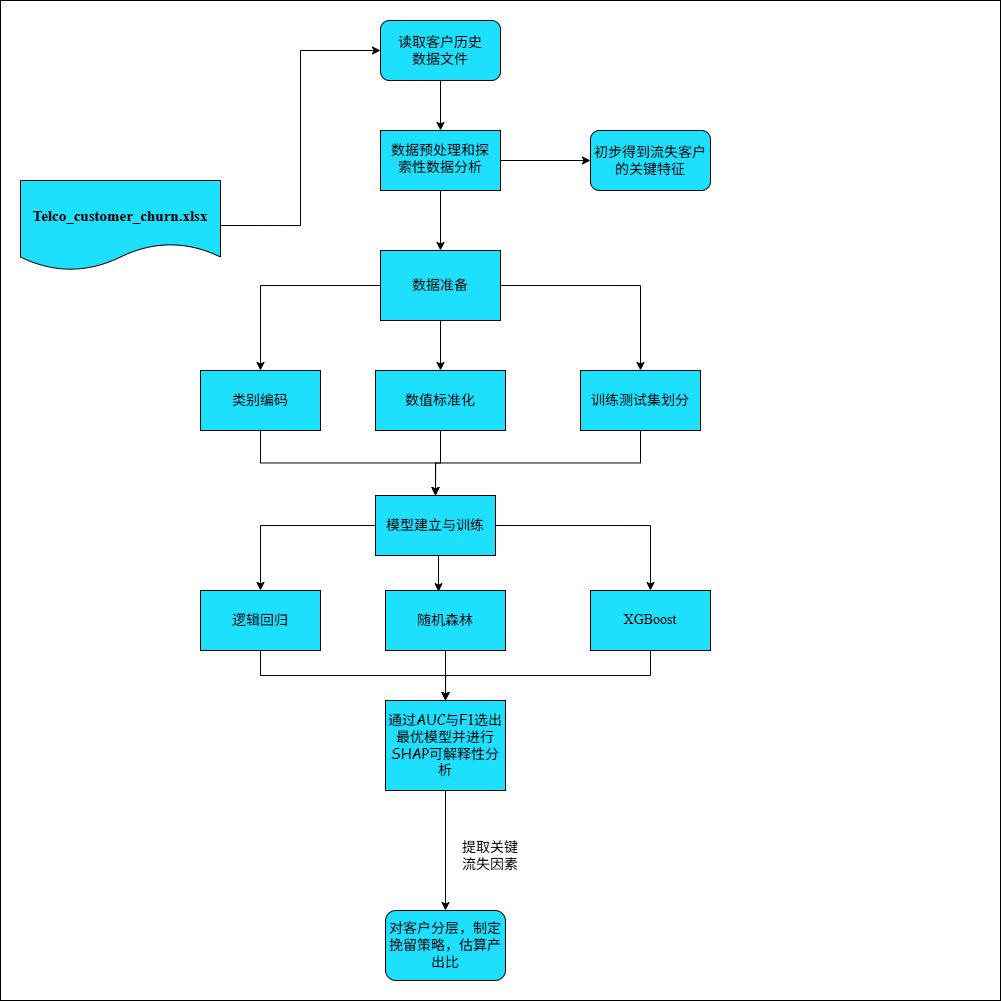
\includegraphics[width=0.8\textwidth]{flowchart.png}
    \fbox{\parbox{0.6\textwidth}{\centering\vspace{3cm}（在此插入流程图）\vspace{3cm}}}
    \caption{整体建模流程图}
    \label{fig:flowchart}
\end{figure}

首先进行数据预处理（数据清洗、标准化等），然后依次针对三个子问题建立模型并求解，最后对模型进行检验和评价。

\section{模型假设与符号说明}

\subsection{模型假设}

为在可处理的框架内抓住问题的核心矛盾，本文作以下约定：

\begin{enumerate}
    \item \textbf{样本代表性。}所给 7043 条记录能代表该运营商的客户总体，
    不存在系统性的抽样偏倚。
    \item \textbf{客户独立应答。}不同客户的离网决策彼此独立，
    排除同一家庭成员间的联动退订效应。
    \item \textbf{特征充分性。}现有字段已覆盖客户流失的主要诱因，
    未被记录的宏观因素（竞争环境、经济波动等）的残余影响较小。
    \item \textbf{标注可靠。}Churn Value 字段如实记录了客户的留存/离网状态，
    无误标或漏标。
    \item \textbf{行为稳态。}考察期内客户的消费模式与服务使用强度
    未发生剧烈变动，可近似视为平稳。
\end{enumerate}

\subsection{符号说明}

本文使用的主要符号及其含义如表 \ref{tab:notation} 所示。

\begin{table}[htbp]
    \centering
    \caption{主要符号说明}
    \label{tab:notation}
    \small
    \begin{tabular}{ccl}
        \toprule
        {\heiti 符号} & {\heiti 单位} & {\heiti 含义} \\
        \midrule
        \multicolumn{3}{l}{\heiti\small （一）数据与特征} \\
        $N$        & -- & 样本总数（7043） \\
        $p$        & -- & 编码后特征维度（31） \\
        $x_i$      & -- & 第 $i$ 个样本的特征向量 \\
        $y_i$      & -- & 第 $i$ 个样本的流失标签（$0/1$） \\
        $r$        & -- & Pearson 线性相关系数 \\
        \addlinespace
        \multicolumn{3}{l}{\heiti\small （二）逻辑回归模型} \\
        $P$        & -- & 模型输出的流失概率 $\in (0,1)$ \\
        $\hat{y}_i$ & -- & 第 $i$ 个样本的预测类别 \\
        $\beta_0$  & -- & 截距项（偏置） \\
        $\beta_j$  & -- & 第 $j$ 个特征的回归系数 \\
        $\lambda$  & -- & $\ell_2$ 正则化强度 \\
        \addlinespace
        \multicolumn{3}{l}{\heiti\small （三）评估与验证} \\
        AUC        & -- & ROC 曲线下面积 \\
        F1         & -- & 精确率与召回率的调和均值 \\
        $k$        & -- & 交叉验证折数 \\
        \addlinespace
        \multicolumn{3}{l}{\heiti\small （四）可解释性与分层} \\
        $\phi_j$   & -- & 第 $j$ 个特征的 SHAP 值 \\
        $P_{50}$   & -- & 预测概率的第 50 百分位数 \\
        $P_{80}$   & -- & 预测概率的第 80 百分位数 \\
        \addlinespace
        \multicolumn{3}{l}{\heiti\small （五）策略评估} \\
        CLTV       & -- & 客户生命周期价值（美元） \\
        $R_{\text{reach}}$ & -- & 挽留方案的触达率 \\
        $R_{\text{retain}}$ & -- & 触达客户的挽留成功率 \\
        \bottomrule
    \end{tabular}
\end{table}

\section{问题一：流失客户画像构建}

\subsection{数据预处理}

原始数据来自题目附件 Telco\_customer\_churn.xlsx，共 7043 条记录、33 个字段，涵盖客户人口统计学信息、账户信息、服务订阅信息和流失标签。

首先对数据进行清洗。剔除 CustomerID、Count、Country 三列：
CustomerID 作为唯一标识，与客户流失情况无关，无泛化预测能力；
Count 恒为 1，方差为 0，对区分客户无贡献；
Country 全部为 United States，无差异性，对模型无额外信息量。

其次，经检查 \texttt{Total Charges} 列为字符串类型。
经 \texttt{pd.to\_numeric}
转换后确认 11 条 \texttt{NaN} 记录。追溯发现这 11 条记录的
\texttt{Tenure Months} 均为 0（新客户尚未产生消费），因此填充为 0，
符合正常业务逻辑。处理后全部 7043 行无缺失值。

为便于后续分析中引用，表 \ref{tab:variable_mapping} 按业务类别
整理了关键变量的中英文名称对照及类别归属。后续分析将围绕表中所列的
时长与费用、合同与支付、服务订阅、人口与家庭四大维度展开。

\begin{table}[H]
    \centering
    \caption{关键变量名称对照表}
    \label{tab:variable_mapping}
    \small
    \begin{tabular}{clll}
        \toprule
        {\heiti 变量类别} & {\heiti 中文名称}
        & {\heiti 原始列名} & {\heiti 说明} \\
        \midrule
        目标变量 & 是否流失 & Churn Value
        & 1=流失, 0=未流失 \\
        \addlinespace
        \multicolumn{4}{l}{\heiti \small （一）时长与费用特征} \\
        数值 & 在网时长 & Tenure Months & 单位：月 \\
        数值 & 月消费金额 & Monthly Charges & 单位：美元 \\
        数值 & 总消费金额 & Total Charges & 单位：美元 \\
        数值 & 客户生命周期价值 & CLTV & Customer Lifetime Value \\
        \addlinespace
        \multicolumn{4}{l}{\heiti \small （二）合同与支付特征} \\
        分类 & 合同类型 & Contract & 月付/一年/两年 \\
        分类 & 支付方式 & Payment Method & 共 4 种 \\
        二分类 & 是否无纸化账单 & Paperless Billing & Yes / No \\
        \addlinespace
        \multicolumn{4}{l}{\heiti \small （三）服务订阅特征} \\
        多分类 & 互联网服务类型 & Internet Service & DSL/Fiber optic/No \\
        二分类 & 在线安全服务 & Online Security & Yes/No/No internet \\
        二分类 & 技术支持服务 & Tech Support & Yes/No/No internet \\
        \addlinespace
        \multicolumn{4}{l}{\heiti \small （四）人口与家庭特征} \\
        二分类 & 是否老年人 & Senior Citizen & Yes / No \\
        二分类 & 是否有配偶 & Partner & Yes / No \\
        二分类 & 是否有家属 & Dependents & Yes / No \\
        \addlinespace
        \multicolumn{4}{l}{\heiti \small （五）其他说明} \\
        文本 & 客户编号 & CustomerID & 无预测价值，已剔除 \\
        数值 & 纬度 & Latitude & 与流失相关系数<0.01 \\
        数值 & 经度 & Longitude & 与流失相关系数<0.01 \\
        \bottomrule
    \end{tabular}
\end{table}

\subsection{流失客户特征探索}

\subsubsection*{整体流失率}

以 Churn Value 为分类依据进行统计，流失客户 $1869$ 人，未流失客户
$5174$ 人，总客户 $7043$ 人，整体流失率为 $26.54\%$，如图
\ref{fig:churn_rate} 所示。

\begin{figure}[H]
    \centering
    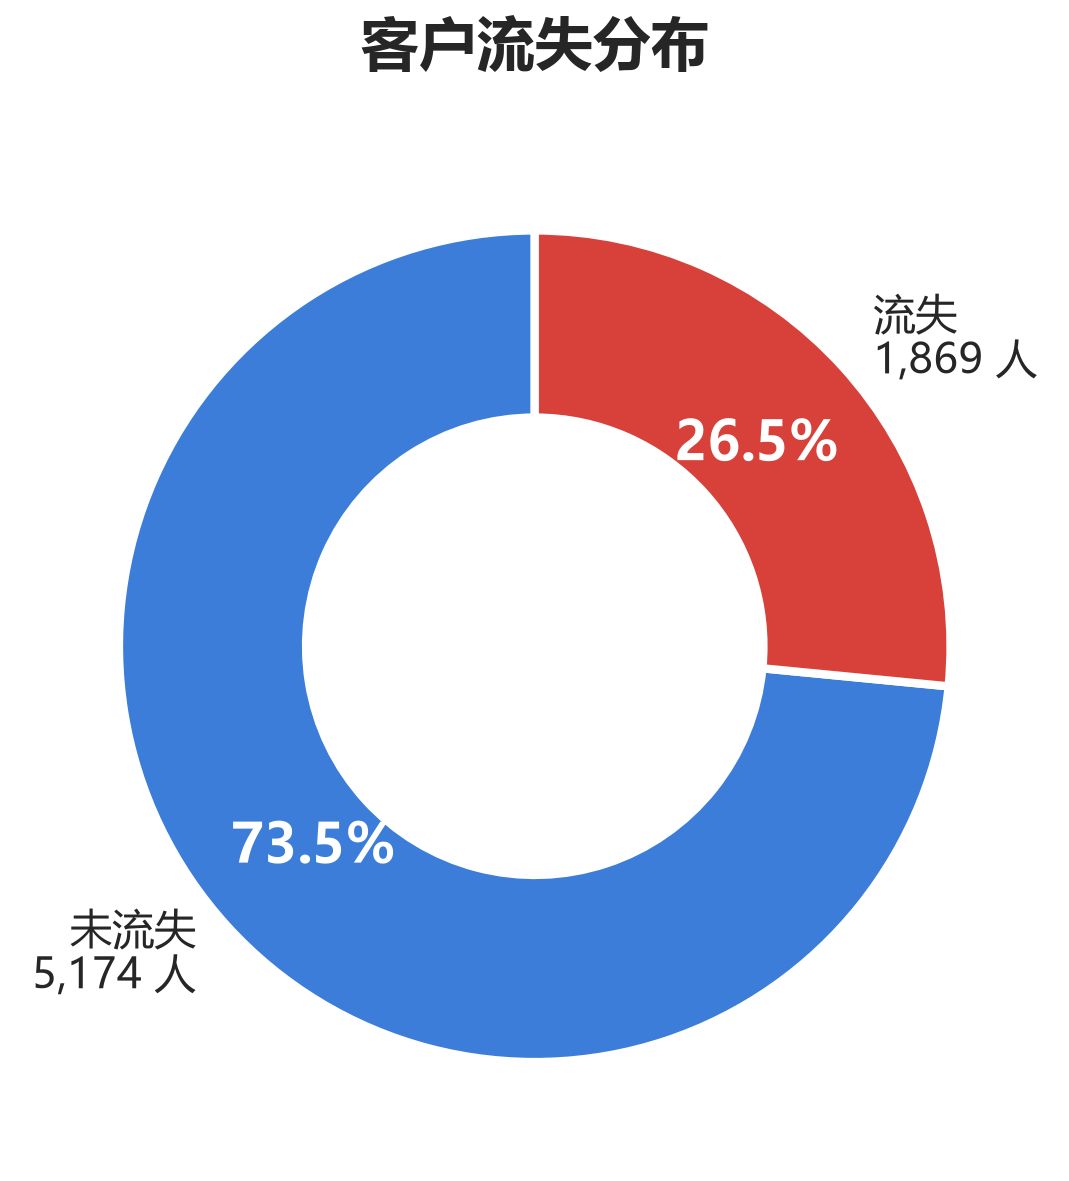
\includegraphics[width=0.5\textwidth]{figures/整体流失率.png}
    \caption{整体流失率环形图}
    \label{fig:churn_rate}
\end{figure}

从分布比例来看，流失与未流失两类样本的比例约为 1:2.8，呈现一定程度的
类别不均衡。这一比例虽然不属严重失衡（如 1:10 以上），但已足以对常规
分类模型的训练过程产生影响——模型倾向于将多数类（未流失）识别得更好
以降低整体损失，而牺牲对少数类（流失）的识别能力。
例如，一个将所有样本都预测为"未流失"的简单模型也能获得 $73.46\%$
的准确率，但这显然不能反映模型在实际业务中的价值。

为此，后续建模中评价指标弃用对类别比例敏感的准确率，
转为采用 AUC 和 F1-score；训练时对逻辑回归设置
\texttt{class\_weight='balanced'} 参数，按类别频数自动调整损失权重，
强化对流失客户的关注。

\subsubsection*{数值特征分布对比}

为考察流失与未流失客户在数值特征上的分布差异，选取在网时长（Tenure Months）、
月消费金额（Monthly Charges）和总消费金额（Total Charges）
三个核心数值特征，分别绘制分组直方图与箱线图，如图 \ref{fig:num_features}
所示。

\begin{figure}[H]
    \centering
    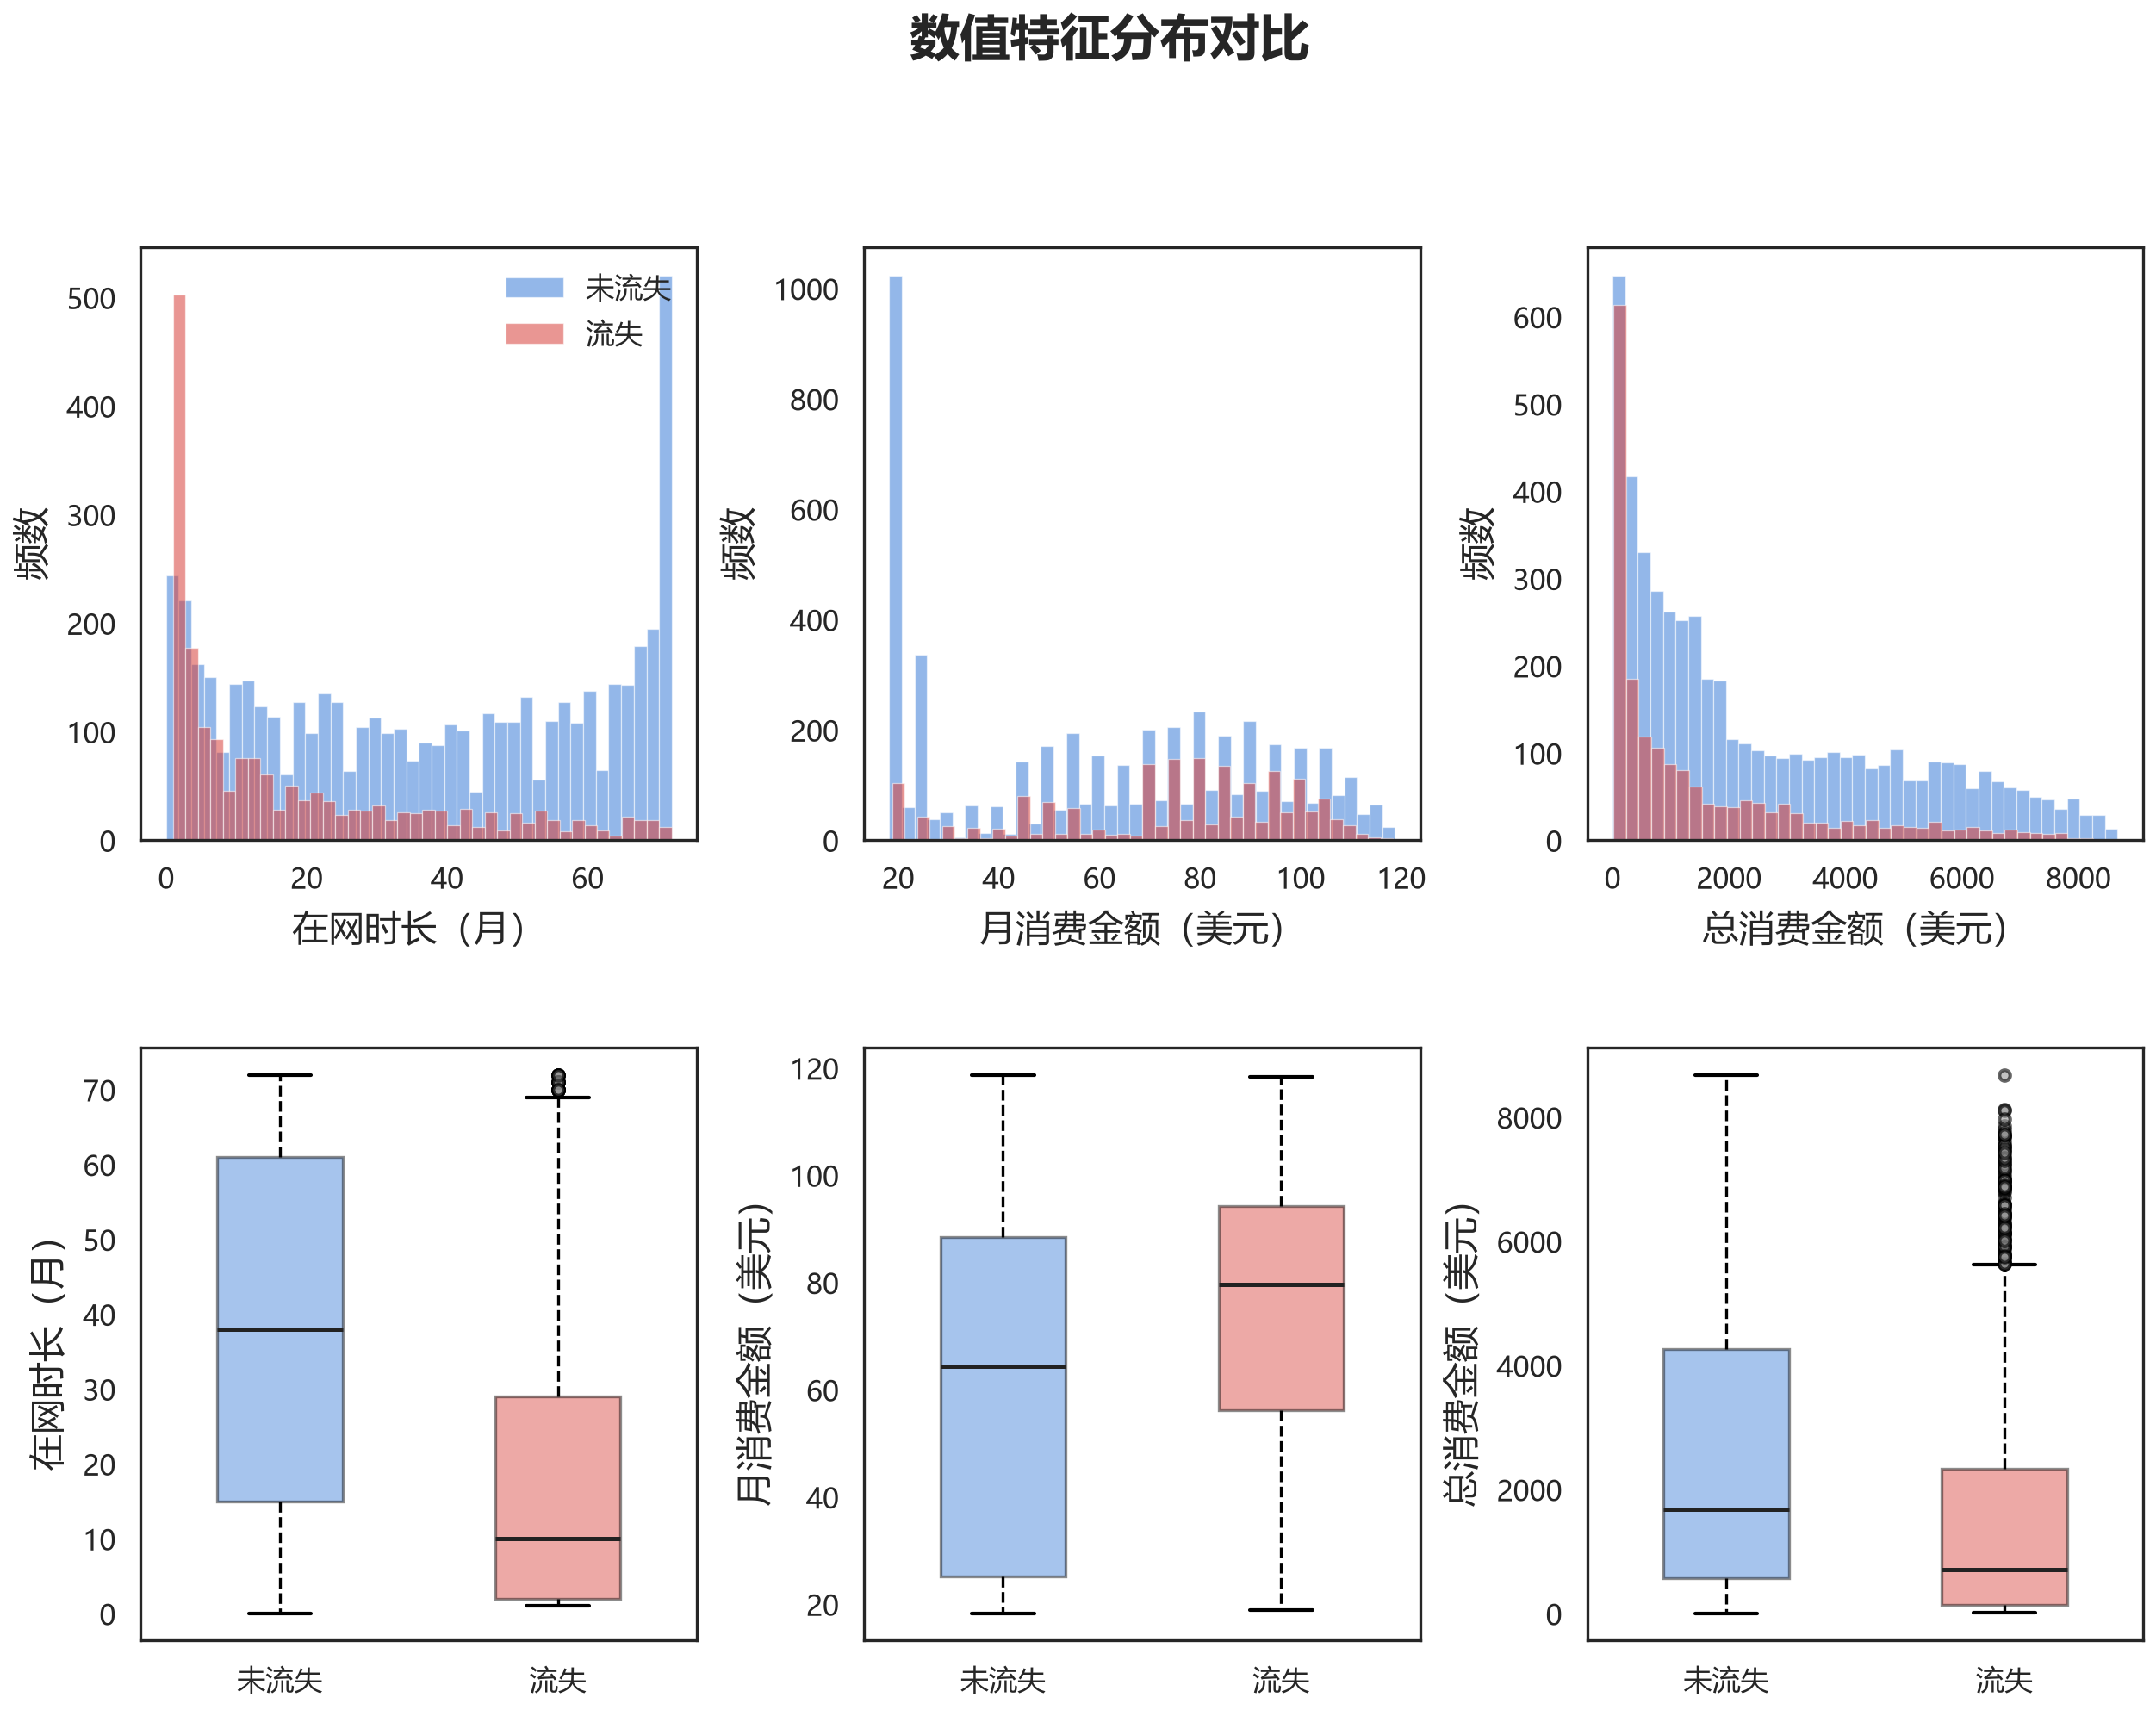
\includegraphics[width=0.85\textwidth]{figures/数值特征分布对比.png}
    \caption{数值特征分布对比图}
    \label{fig:num_features}
\end{figure}

由直方图和箱线图可以观测到以下规律：

\textbf{在网时长：}流失客户的分布高度集中于 0-10 个月的低在网时长区间，
而未流失客户的分布较为均匀，覆盖 0-72 个月的全区间。箱线图显示两组
中位数差距显著，说明在网时长是区分能力最强的数值特征——新客户是流失的
高风险群体。

\textbf{月消费金额：}流失客户的月消费整体偏高，在 70-110 美元的高费区间
聚集密度明显大于未流失客户。高消费客户对价格更为敏感，流失意愿相对更强。

\textbf{总消费金额：}流失客户的总消费明显偏低且呈左偏分布，但该差异主要
源于在网时长短导致的消费积累不足，属于在网时长的间接效应，
其独立区分能力有限。

综合以上分析，在网时长是区分流失与未流失最有效的数值特征。

\subsubsection*{分类特征流失率对比}

为考察分类变量各取值水平下的流失风险差异，选取合同类型、互联网服务
类型、支付方式、是否老年人、是否有配偶、是否有家属、是否开通电话服务、
是否无纸化账单共 8 个分类特征，分别统计各组流失率并绘制柱状图，
如图 \ref{fig:cat_features} 所示。

\begin{figure}[H]
    \centering
    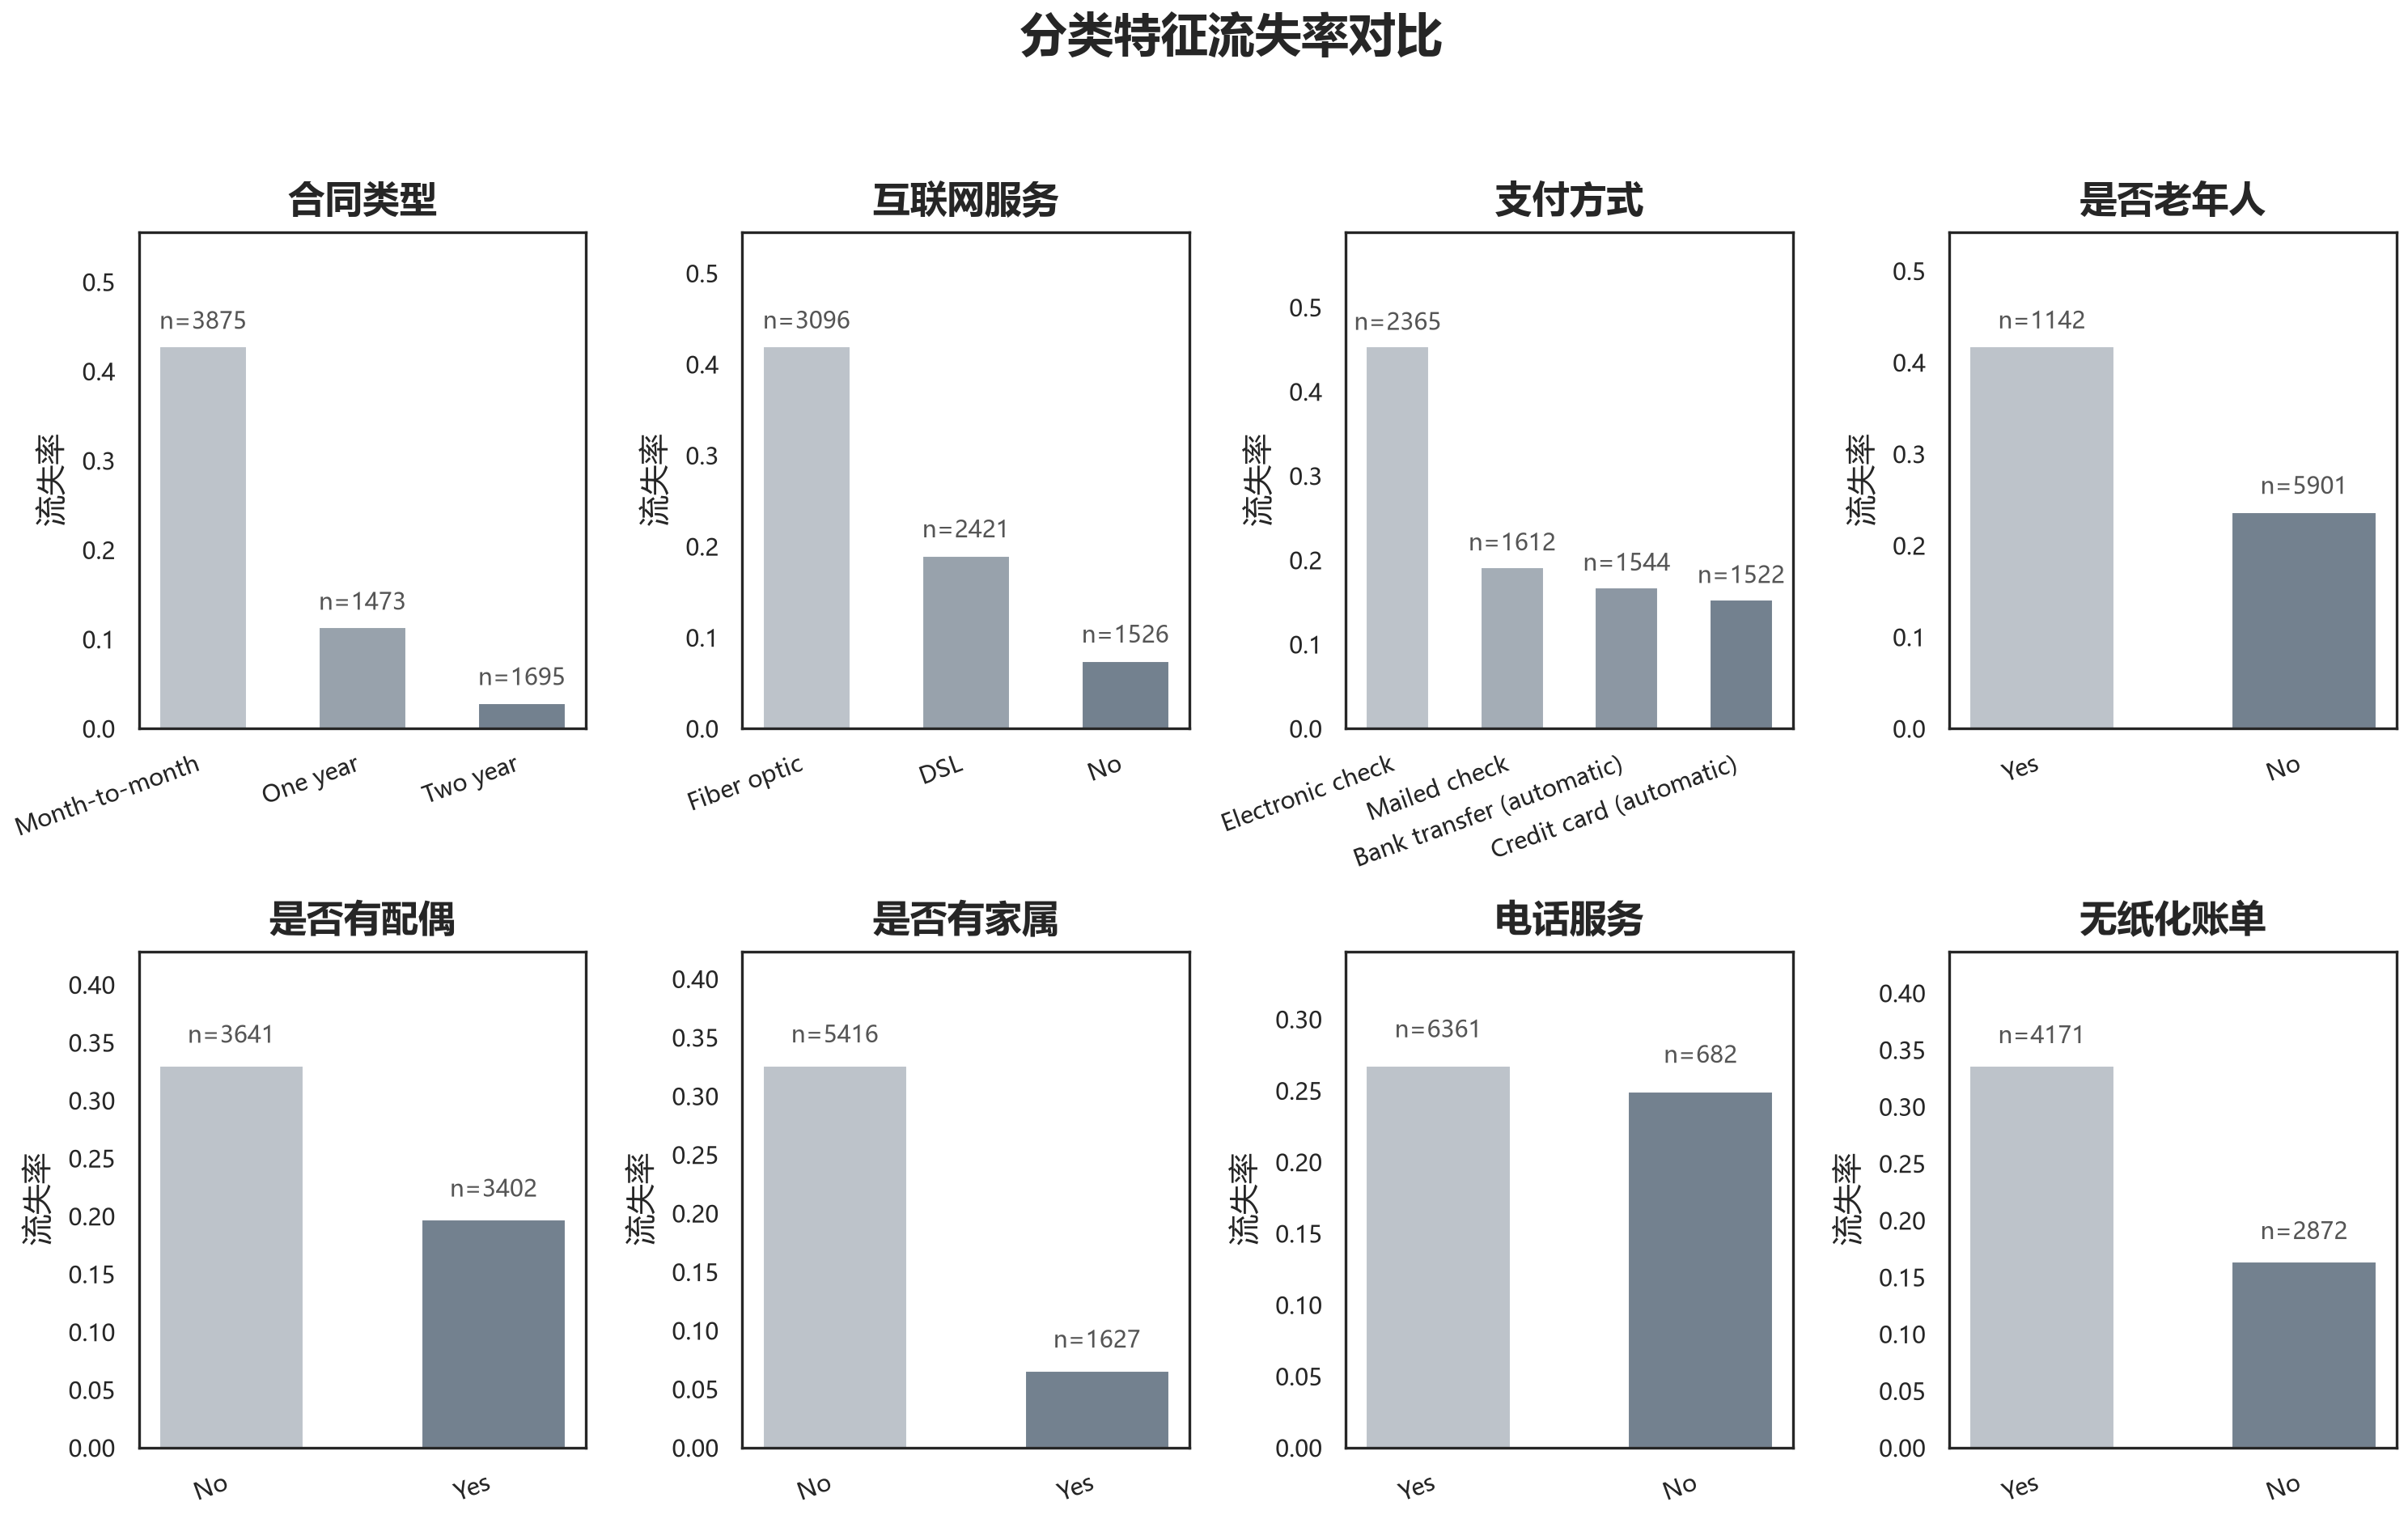
\includegraphics[width=0.85\textwidth]{figures/分类特征流失率对比.png}
    \caption{分类特征流失率对比图}
    \label{fig:cat_features}
\end{figure}

各分类特征的分组流失率如表和图所示，具体分析如下：

\textbf{合同类型（Contract）：}月付合同的流失率超过 40\%，而一年合同
约为 10\%、两年合同约为 3\%。合同期限的差异根本性地改变了客户流失的
转换成本——月付客户可以随时解约，而年付和两年合同的客户通常承担了
提前解约的违约金或已享受合约折扣，转换运营商的意愿显著降低。

\textbf{互联网服务类型（Internet Service）：}光纤客户的流失率显著高于
DSL 客户和无互联网客户，可能与光纤服务的高月费有关——高消费群体对
服务性价比的要求也更高。

\textbf{支付方式（Payment Method）：}电子支票客户的流失率约为 45\%，
而银行自动转账、信用卡自动支付和邮寄支票三种方式的流失率均在
15\%-20\% 之间，表明支付方式与客户属性之间存在一定的关联性。

此外，有配偶或有家属的客户流失率低于独身客户（家庭绑定提高了离网成本），
无纸化账单客户流失率高于纸质账单客户（无纸化账单客户更习惯线上操作，
对运营商的服务切换成本感知较低，更容易比价和更换服务商），而是否老年人
和是否开通电话服务对流失率的影响相对较小。

\subsubsection*{相关性热力图}

采用 Pearson 相关系数衡量各数值特征与流失目标之间的线性关联强度
（取值范围 $[-1, 1]$，绝对值越大线性相关越强）。数值变量的相关系数
矩阵以热力图形式呈现在图 \ref{fig:corr} 中。

\begin{figure}[H]
    \centering
    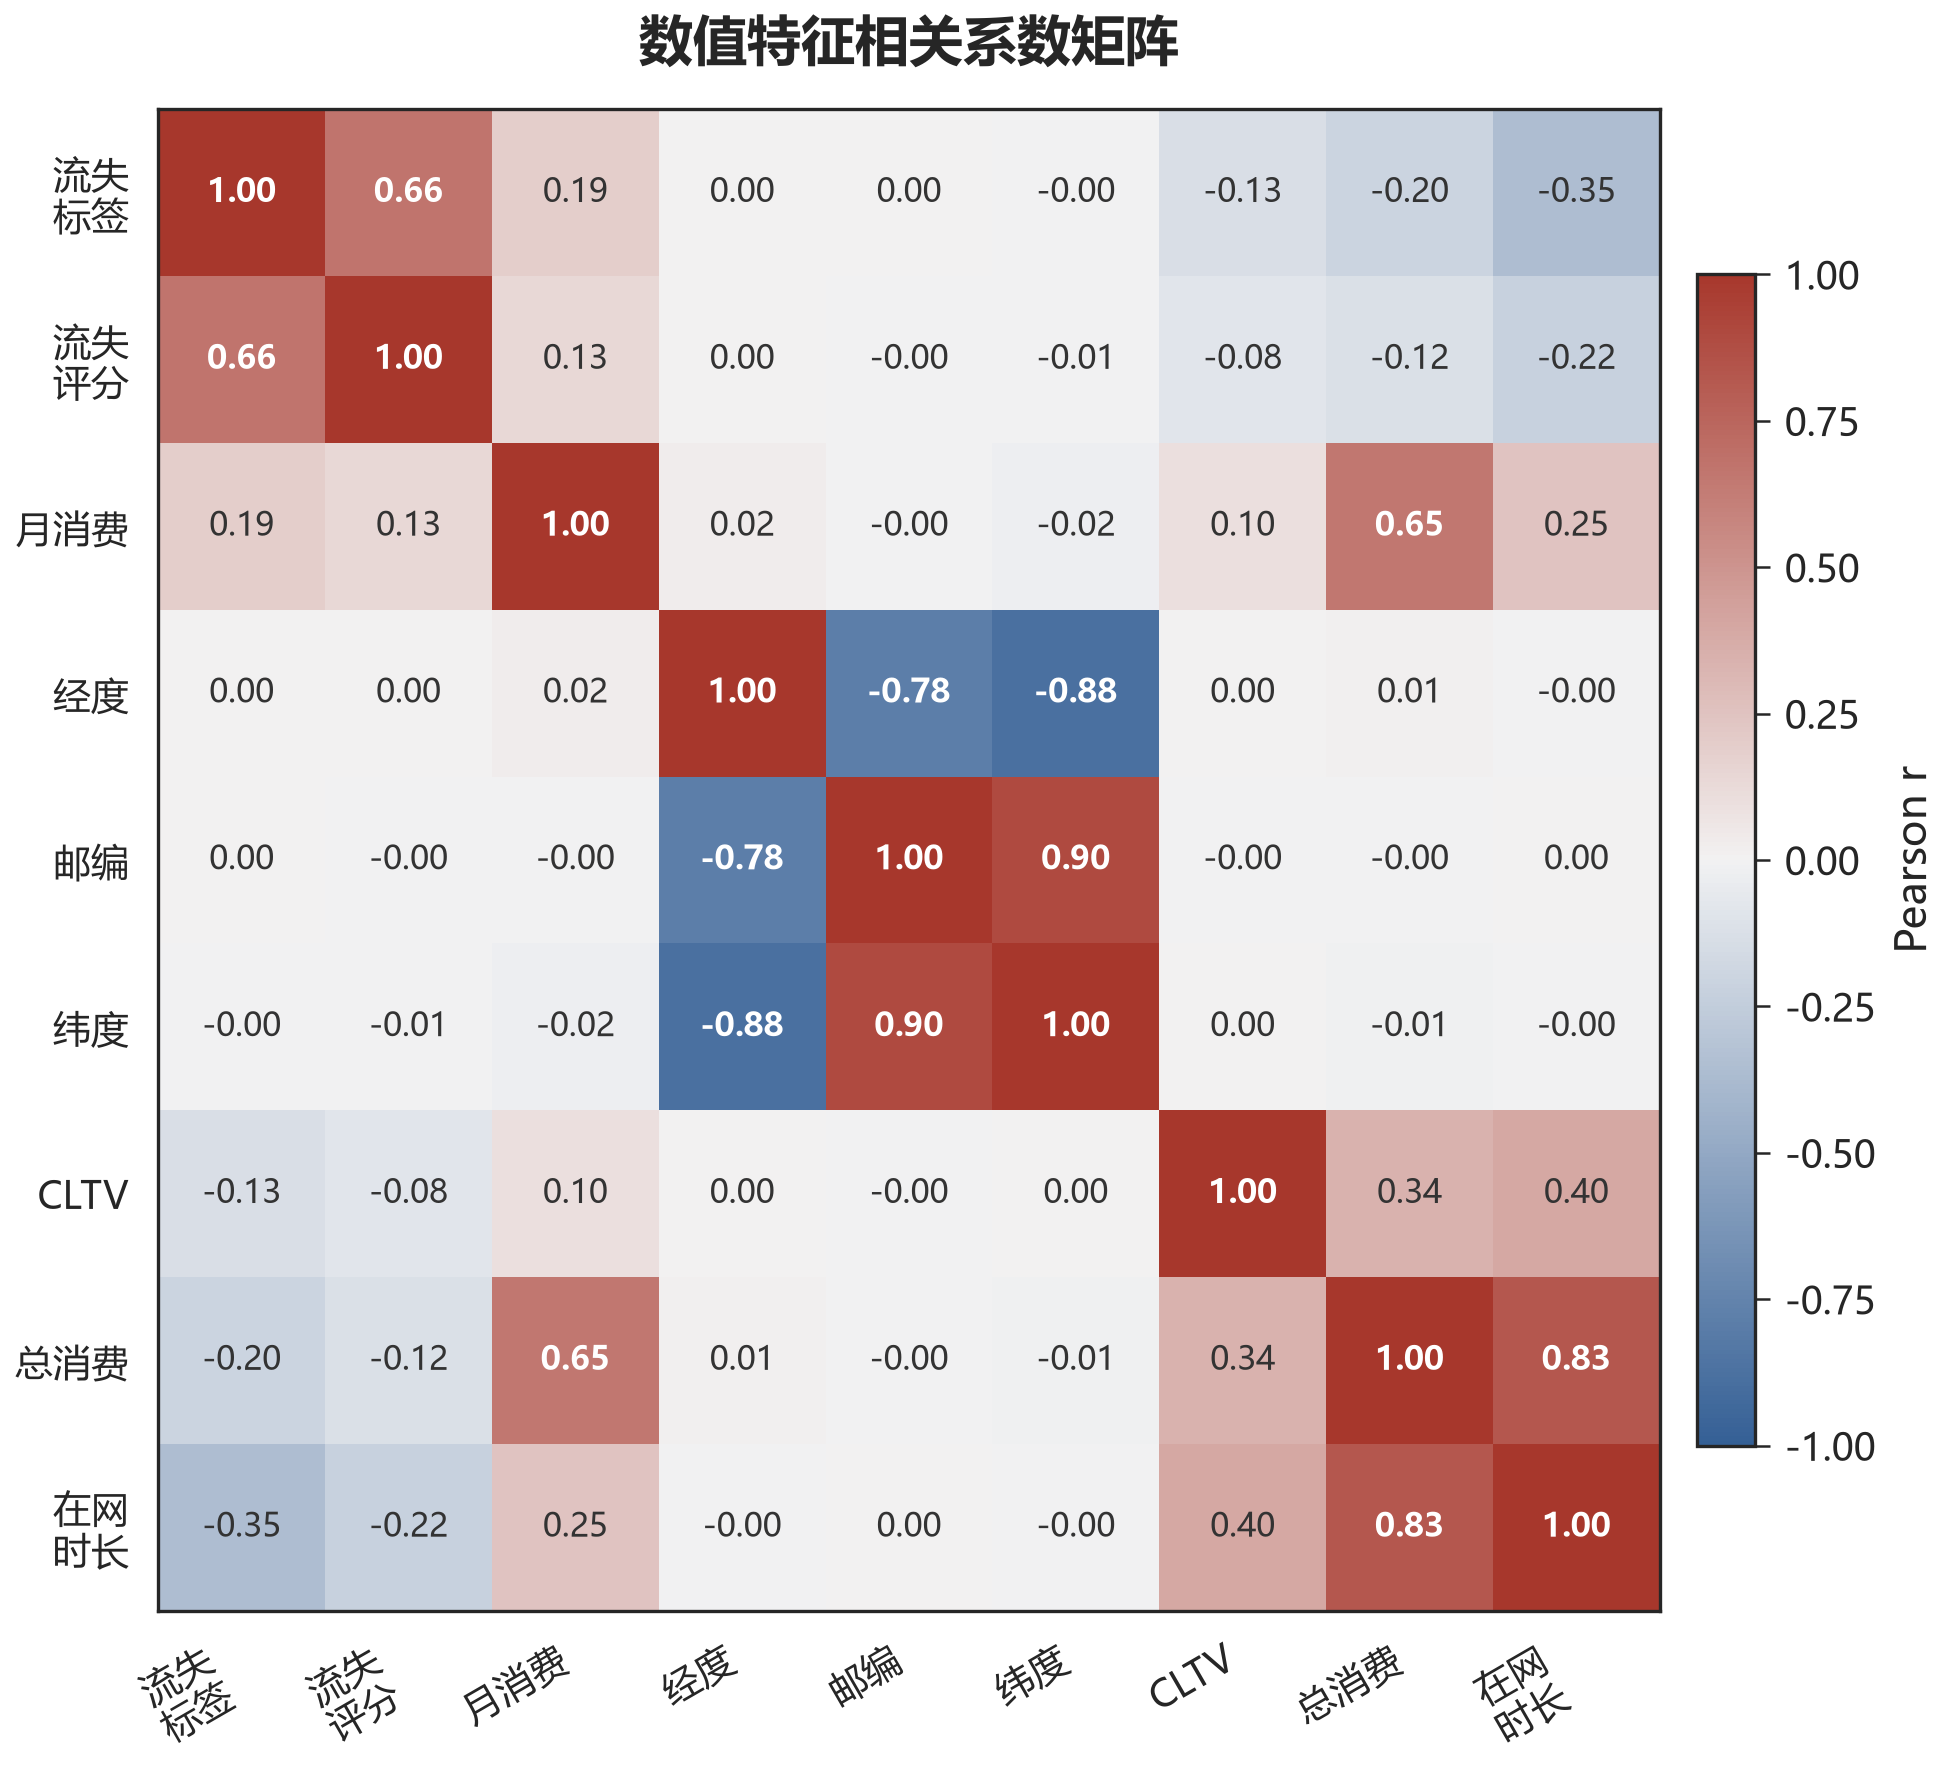
\includegraphics[width=0.75\textwidth]{figures/相关性热力图.png}
    \caption{相关性热力图}
    \label{fig:corr}
\end{figure}

由热力图可见：

\textbf{在网时长：}与流失的相关系数为 $-0.35$，在所有数值特征中
绝对值最大，呈中等程度的负相关——在网时间越长，流失可能性越低，
这与前文分析中"新客户是高危群体"的结论相一致。

\textbf{月消费金额：}与流失的相关系数为 $+0.19$，呈弱正相关——
月消费越高的客户对服务性价比的要求也越高，流失意愿更强，这与分类
特征分析中光纤客户流失率较高的发现互为印证。

\textbf{总消费金额与CLTV：}与流失的相关系数分别为 $-0.20$ 和
$-0.13$，均为弱负相关，方向符合预期。但值得注意的是，在网时长与
总消费之间存在较强的正相关（$r = 0.83$），这是因为在网时间越长累计
消费自然越高，说明两变量存在多重共线性，后续建模中可考虑择一保留。

\textbf{地理特征：}经度、纬度、邮编三个特征与流失的相关系数绝对值
均小于 $0.01$，不具备线性预测价值，说明地理位置与客户的流失决策之间
不存在明显的关联关系。

\subsection{初步结论}

综合上述探索性分析，可从以下维度刻画流失客户的典型特征：
在合同层面，流失客户以月付合同为主，其流失率超过 40\%，
远高于年付和两年合同客户；在在网时长层面，流失客户高度集中在
在网 0-10 个月的新客户群体，在网时长是与流失相关性最强的数值特征
（$r = -0.35$）；在消费层面，流失客户的月消费金额偏高，
高消费群体对服务性价比更为敏感，流失意愿更强；
在家庭层面，无配偶、无家属的独身客户流失率高于有家庭绑定的客户，
前者离网成本更低。

上述发现为下一节分类模型的建立提供了明确的方向：
模型应重点纳入合同类型、在网时长、月消费金额等具有强区分能力的特征变量；
而地理信息（经纬度、邮编）因相关系数绝对值均低于 $0.01$ 可预先剔除，
从而减少模型维度并降低噪声干扰。

\section{问题二：流失预测模型与关键因子识别}

在问题一构建的流失客户画像基础上，本节的目标是建立一个能够
量化各特征对流失风险的贡献程度的预测模型，以回答题目提出的
核心问题：哪些因素是驱动客户流失的关键原因？为此，
本文按"数据准备 → 模型建立 → 模型验证与对比 → 关键因子识别"
四个阶段依次推进。

\subsection{数据准备}

在进入建模之前，需将问题一中清洗后的原始数据转换为分类模型
可接受的数值格式。按以下三步依次进行。

\subsubsection*{特征筛选}

基于问题一的 EDA 结论和特征自身的性质，剔除四类无建模价值的列：
与目标变量等价的冗余列（Churn Label）、基于已知流失信息计算的
泄露列（Churn Score，其与 Churn Value 的相关系数高达 0.665）、
仅少数样本有值的单边列（Churn Reason），以及在相关性分析中确认
与流失无线性关联的地理位置列（Latitude、Longitude、Lat Long、
State、City、Zip Code，相关系数均小于 0.01）。
共剔除 9 列，保留 20 个候选特征。

\subsubsection*{类别编码与数值标准化}

16 个分类特征中，二分类变量（Gender、Senior Citizen、Partner、
Dependents、Phone Service、Paperless Billing）取值仅两种，
直接采用 Label 编码映射为 0/1。多分类变量（Contract、Internet
Service、Payment Method、Multiple Lines、Online Security、
Online Backup、Device Protection、Tech Support、Streaming TV、
Streaming Movies）各取值之间不存在天然的序关系——例如合同类型
"月付、一年、两年"只是三类不同期限，并非等距的顺序尺度——
因此不宜使用 Label 编码，而是采用 One-Hot 编码并设置
\texttt{drop\_first=True} 以避免多重共线性。
编码后特征维度由 20 列扩展为 31 列。

4 个数值特征（Tenure Months、Monthly Charges、Total Charges、
CLTV）的量纲和取值范围各不相同。为使各特征在模型训练中
得到平等对待、消除量纲差异的影响，本文采用 Z-score 标准化
将各数值特征的均值和标准差分别调整为 0 和 1。

\subsubsection*{数据集划分}

按 8:2 比例划分训练集与测试集。划分时设置
\texttt{stratify=y}，保证两边的流失率保持一致（均为 26.54\%）。
最终得到训练集 5634 条、测试集 1409 条，编码后的特征维度
为 31 列。

至此，原始数据已转化为包含 31 个标准化特征的数值矩阵，
可输入分类模型进行训练和评估。

\subsection{逻辑回归模型建立}

\subsubsection*{Step 1：模型选择与原理}

逻辑回归（Logistic Regression）是二分类问题中应用最广泛的
统计学习方法之一 \cite{li2019statistical}。它的输出值严格
介于 0 和 1 之间，可解释为样本属于正类的概率，且每个特征的
回归系数 $\beta_j$ 直接反映了该特征对流失概率的影响方向
（系数符号）与强度（绝对值大小），这使得逻辑回归在需要向
非技术背景的业务方解释建模结论时具有天然优势。

本文优先采用逻辑回归作为基线模型，主要基于两点考虑。
第一，问题一的 EDA 已表明流失与各特征之间以线性关系为主：
在网时长与流失的相关系数为 $-0.352$，月消费金额为 $+0.193$，
而更为复杂的非线性交互信号并不突出。第二，问题二的核心要求
不仅在于预测精度，更在于识别关键流失因素并给出合理的业务解释，
逻辑回归的系数可解释性恰好满足这一要求。

逻辑回归假设客户流失概率 $P(Y=1 \mid X)$ 满足 Sigmoid 函数映射：
\begin{equation}
    P(Y=1 \mid X)
    = \frac{1}{1 + e^{-(\beta_0 + \beta_1 x_1 + \cdots + \beta_p x_p)}}
    \label{eq:sigmoid}
\end{equation}
其中 $\beta_0$ 为截距项，$\beta_j$ 为第 $j$ 个特征的回归系数。
模型的参数通过最大化带 $\ell_2$ 正则化的对数似然函数来估计：
\begin{equation}
    \ell = \sum_{i=1}^{N} \left[
        y_i \ln P_i + (1 - y_i) \ln (1 - P_i)
    \right] - \lambda \|\beta\|^2
    \label{eq:loglik}
\end{equation}

\subsubsection*{Step 2：模型训练}

本文使用 scikit-learn 的 LogisticRegression 实现，
通过求解式 \eqref{eq:loglik} 的对数似然函数完成参数估计。

此外，问题一的整体流失率分析（26.54\%）已确认数据存在类别
不平衡问题。为避免模型在训练中过度偏向多数类（未流失客户），
本文设置 \texttt{class\_weight='balanced'}，使模型根据各类别的
样本数量自动调整损失权重，加大对少数类（流失客户）误判的
惩罚力度。

\subsubsection*{Step 3：模型评估}

逻辑回归在测试集上的预测结果如表 \ref{tab:lr_metrics} 所示。

\begin{table}[H]
    \centering
    \caption{逻辑回归模型评估指标}
    \label{tab:lr_metrics}
    \begin{tabular}{ccccc}
        \toprule
        Accuracy & Precision & Recall & F1-score & AUC \\
        \midrule
        0.742    & 0.51      & 0.78   & 0.62     & 0.849 \\
        \bottomrule
    \end{tabular}
\end{table}

\begin{figure}[H]
    \centering
    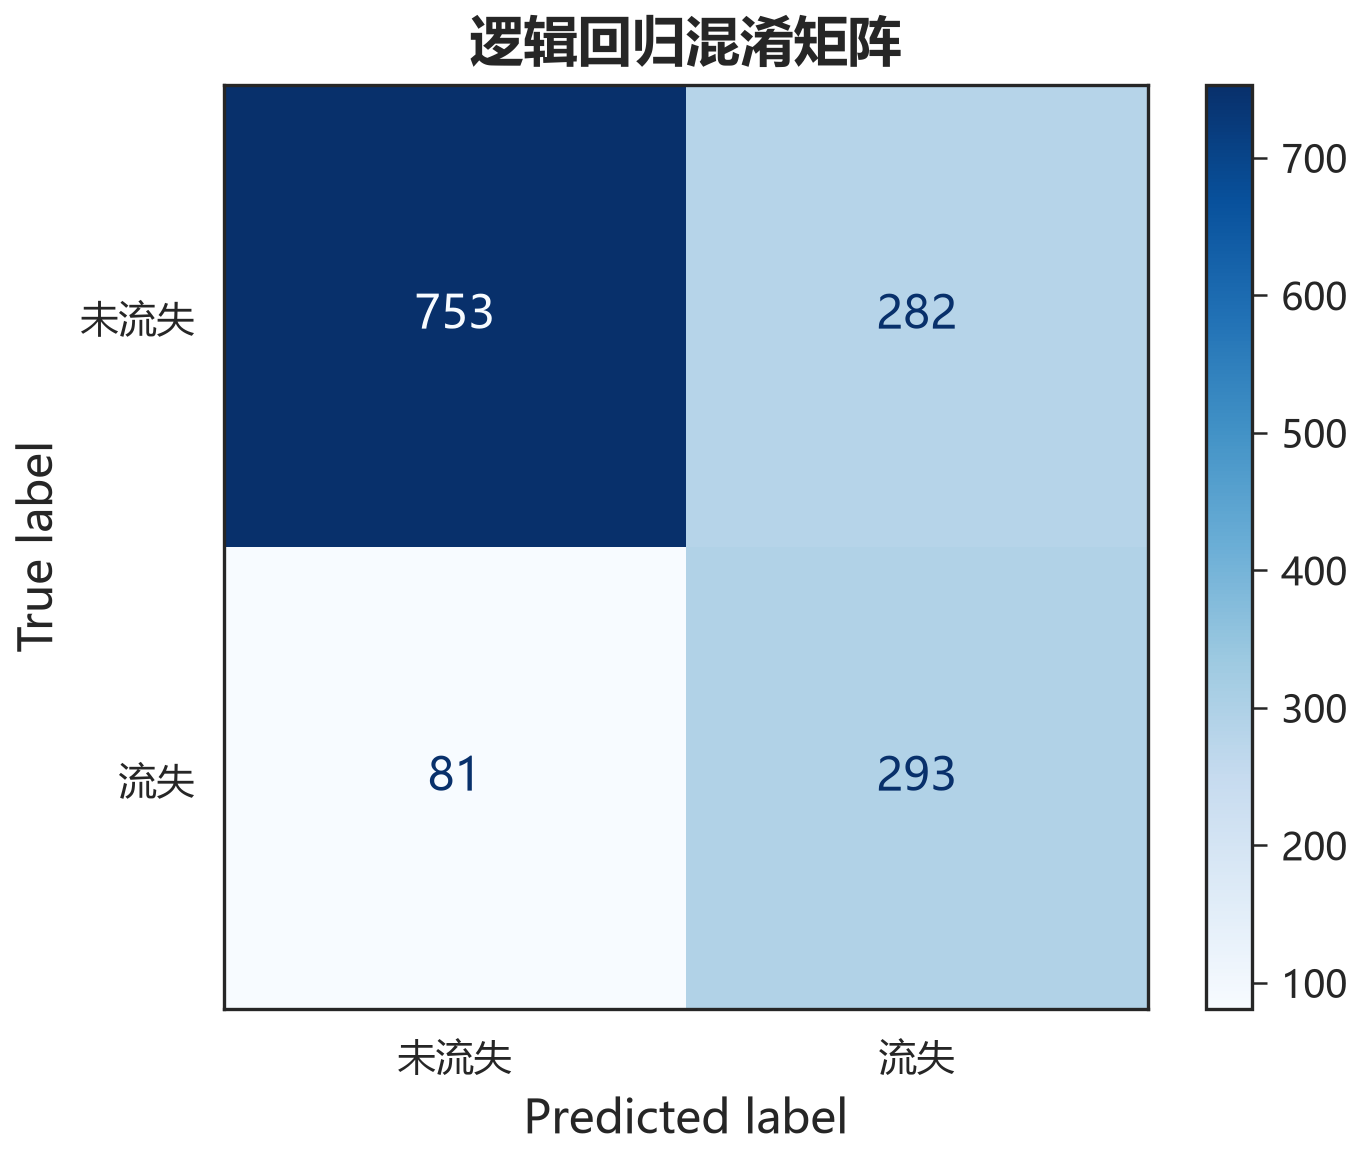
\includegraphics[width=0.5\textwidth]{figures/confusion_matrix.png}
    \caption{逻辑回归混淆矩阵}
    \label{fig:confusion_matrix}
\end{figure}

混淆矩阵的四格分别对应：真阴性（左上，正确预测未流失）、
假阳性（右上，将未流失误判为流失）、假阴性（左下，
将流失误判为未流失）和真阳性（右下，正确预测流失）。
从图中可以看出，模型对未流失客户的分类准确度较高
（左上角数值显著大于右上角），同时得益于
\texttt{class\_weight='balanced'} 的设置，模型也成功识别了
大部分流失客户（右下角），这与表 \ref{tab:lr_metrics} 中
0.78 的召回率相互印证。

\begin{figure}[H]
    \centering
    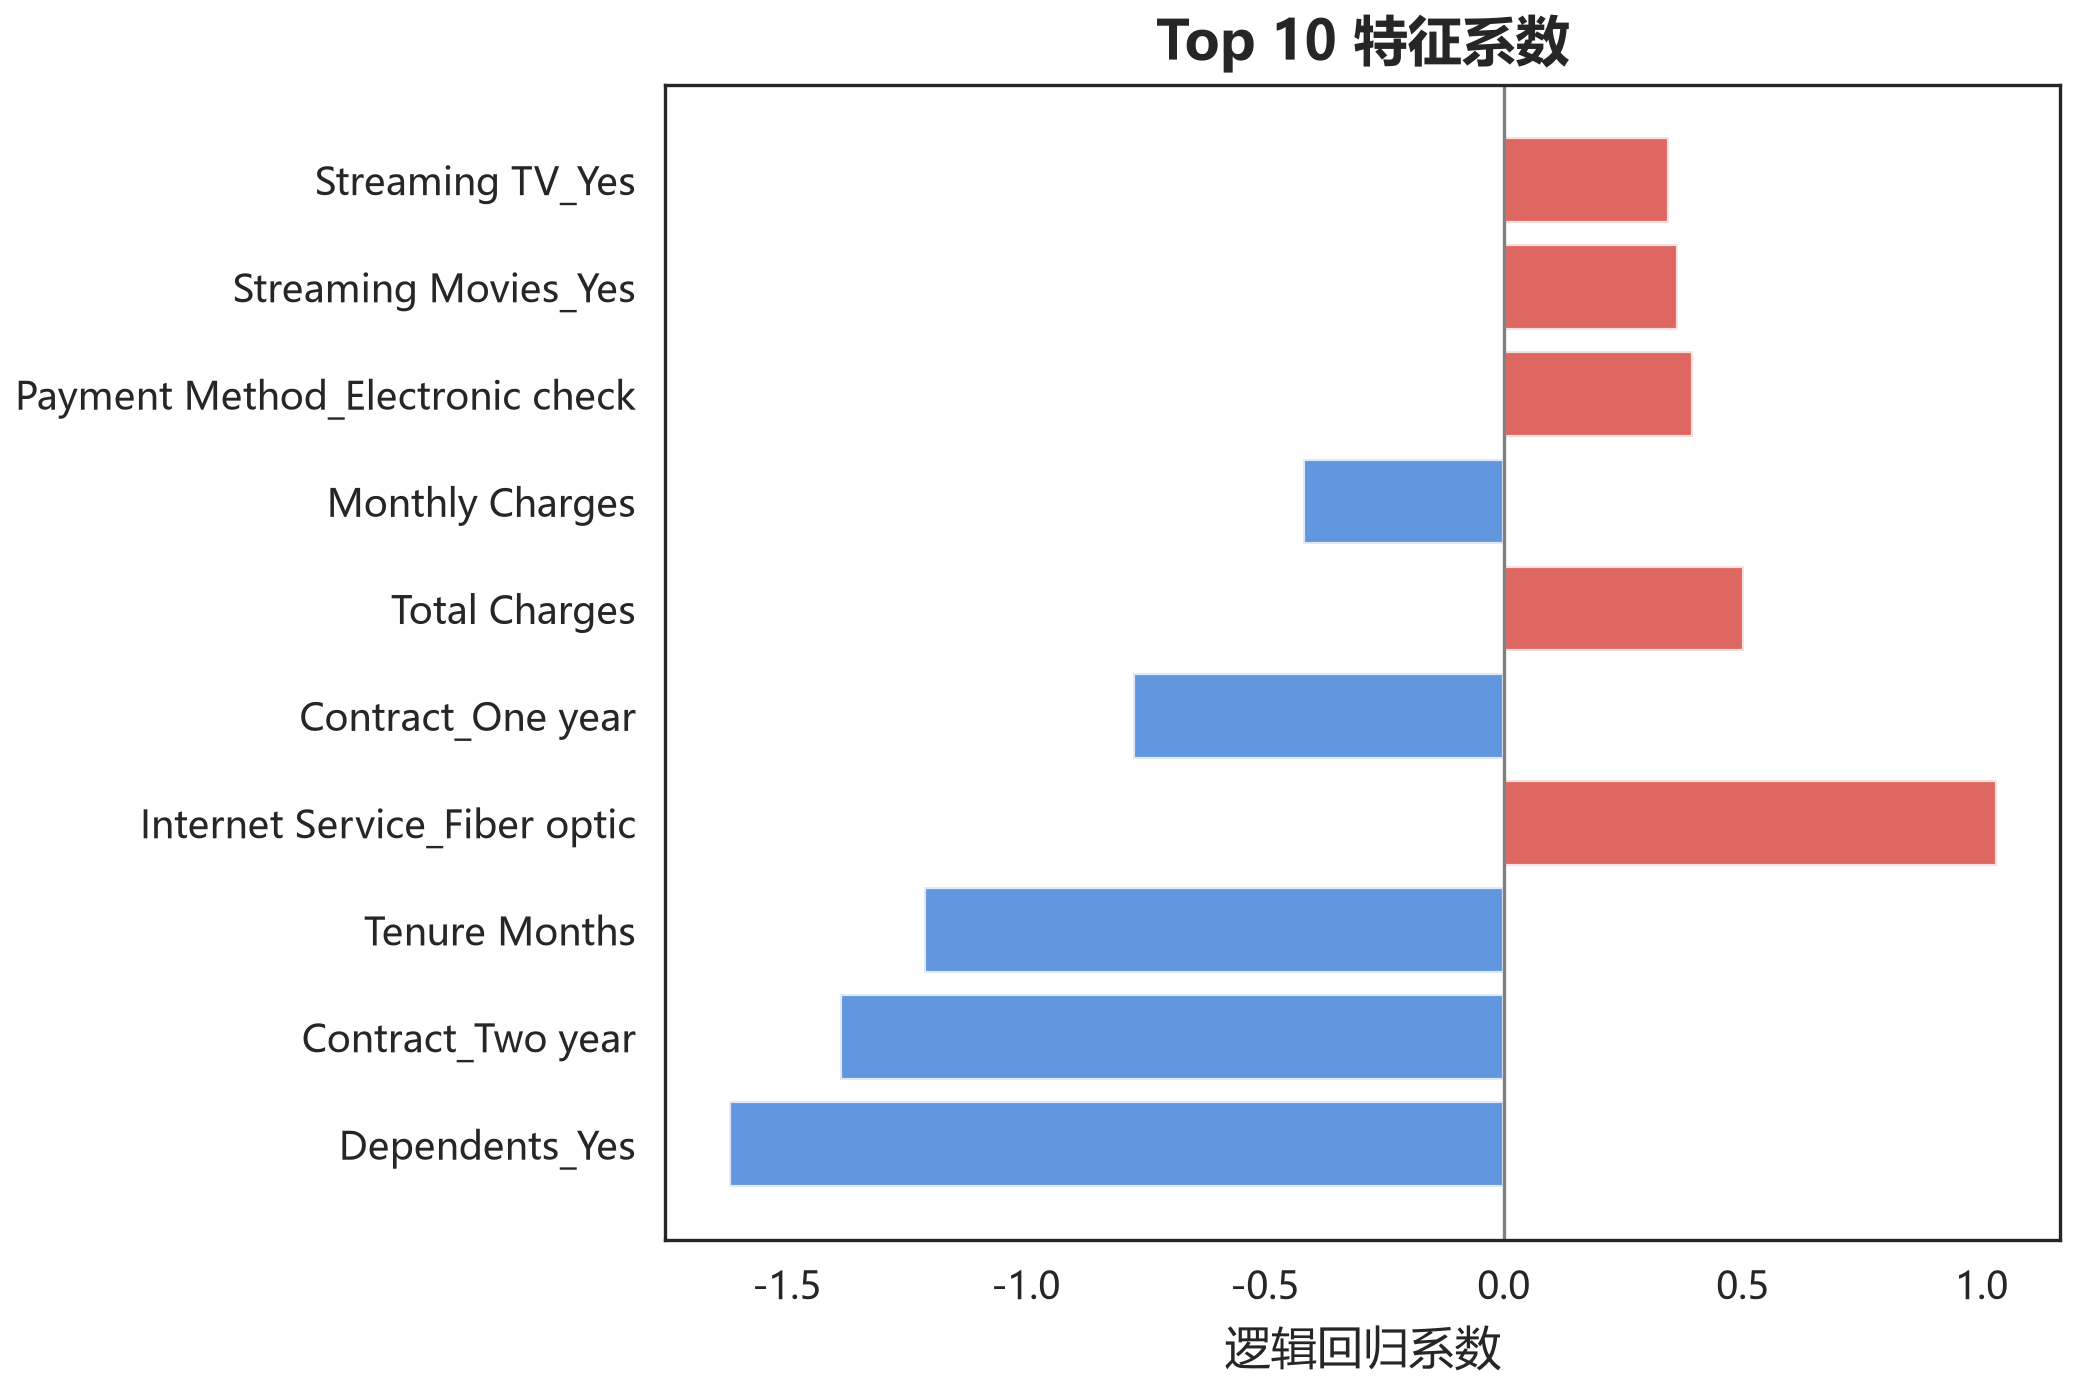
\includegraphics[width=0.65\textwidth]{figures/feature_importance.png}
    \caption{逻辑回归特征系数（Top 10）}
    \label{fig:feature_importance}
\end{figure}

图 \ref{fig:feature_importance} 展示了绝对值最大的前 10 个
逻辑回归系数。蓝色表示负系数——该特征取值增大将降低流失概率，
橙色表示正系数——该特征取值增大将增加流失风险。在网时长的
负系数绝对值最大（约为 $-1.21$），与 EDA 阶段"在网越久越不易
流失"的结论一致；而光纤服务与电子支票支付等特征呈现正系数，
表明这些服务类型本身即关联着较高的流失倾向。需要注意的是，
上述系数受特征间共线性的影响（如在网时长与总消费），
因此仅作为初步参考，更精确的重要性评估将在本节后续通过
SHAP 方法完成。

模型的 AUC 达到 0.849，整体排序能力良好。召回率达到 0.78，
说明模型能够有效识别 78\% 的实际流失客户，具有实用的预警价值。
精确率为 0.51，意味着模型预测为"流失"的客户中约有一半实际
并未流失。从挽留业务的视角来看，误判的代价（向未流失客户
发放挽留优惠）远低于漏判的代价（未能识别出即将流失的客户
而任其离网）。因此，在建模目标上本文优先保证召回率——宁可接受
部分误判带来的额外优惠成本，也要尽可能多地识别出潜在的流失客户，
避免客户离网后更高的替代成本。

\subsection{随机森林与 XGBoost 对比}

随机森林由 Breiman 于 2001 年提出 \cite{breiman2001random}，
其训练过程引入双重随机性——在 Bootstrap 采样的训练子集上，
每棵决策树的分裂仅从随机选取的 $\sqrt{p}$ 个特征中选择最优
分裂点——从而在单棵树容易过拟合的同时，通过集成多棵树的
投票结果获得稳定的整体预测能力。
XGBoost \cite{chen2016xgboost} 是梯度提升树算法的高效实现，
与随机森林并行训练不同，它采用逐轮迭代的方式，使每一棵新树
都去拟合前一棵树的残差，从而逐步降低整体偏差。

仅凭逻辑回归一个模型的评估结果，尚不足以充分判断线性假设
是否已足够刻画该数据集上的流失规律。如果特征之间存在显著的
非线性交互效应，能够捕捉非线性关系的随机森林或 XGBoost
在 AUC 上将明显高于逻辑回归。反之，若三者的 AUC 相近，
则说明线性假设在该问题上是合理的。

\begin{table}[H]
    \centering
    \caption{三模型性能对比}
    \label{tab:model_compare}
    \begin{tabular}{lccc}
        \toprule
        模型 & Accuracy & AUC & F1-score \\
        \midrule
        逻辑回归 & 0.742 & \textbf{0.849} & 0.617 \\
        随机森林 & 0.784 & 0.840 & 0.625 \\
        XGBoost  & 0.750 & 0.847 & 0.622 \\
        \bottomrule
    \end{tabular}
\end{table}

对比结果表明，三者的 AUC 差异不超过 0.01，F1-score 同样高度接近
（均在 0.62 左右）。逻辑回归（AUC=0.849）甚至略高于随机森林
（AUC=0.840）和 XGBoost（AUC=0.847），这说明在该数据集上各特征
与流失概率之间以线性关系为主导，复杂的非线性交互效应并不显著。
因此，逻辑回归不仅具有最强的可解释性，在预测精度上也未因线性
假设的简化而损失性能，适合作为本文的最终预测模型。

\begin{figure}[H]
    \centering
    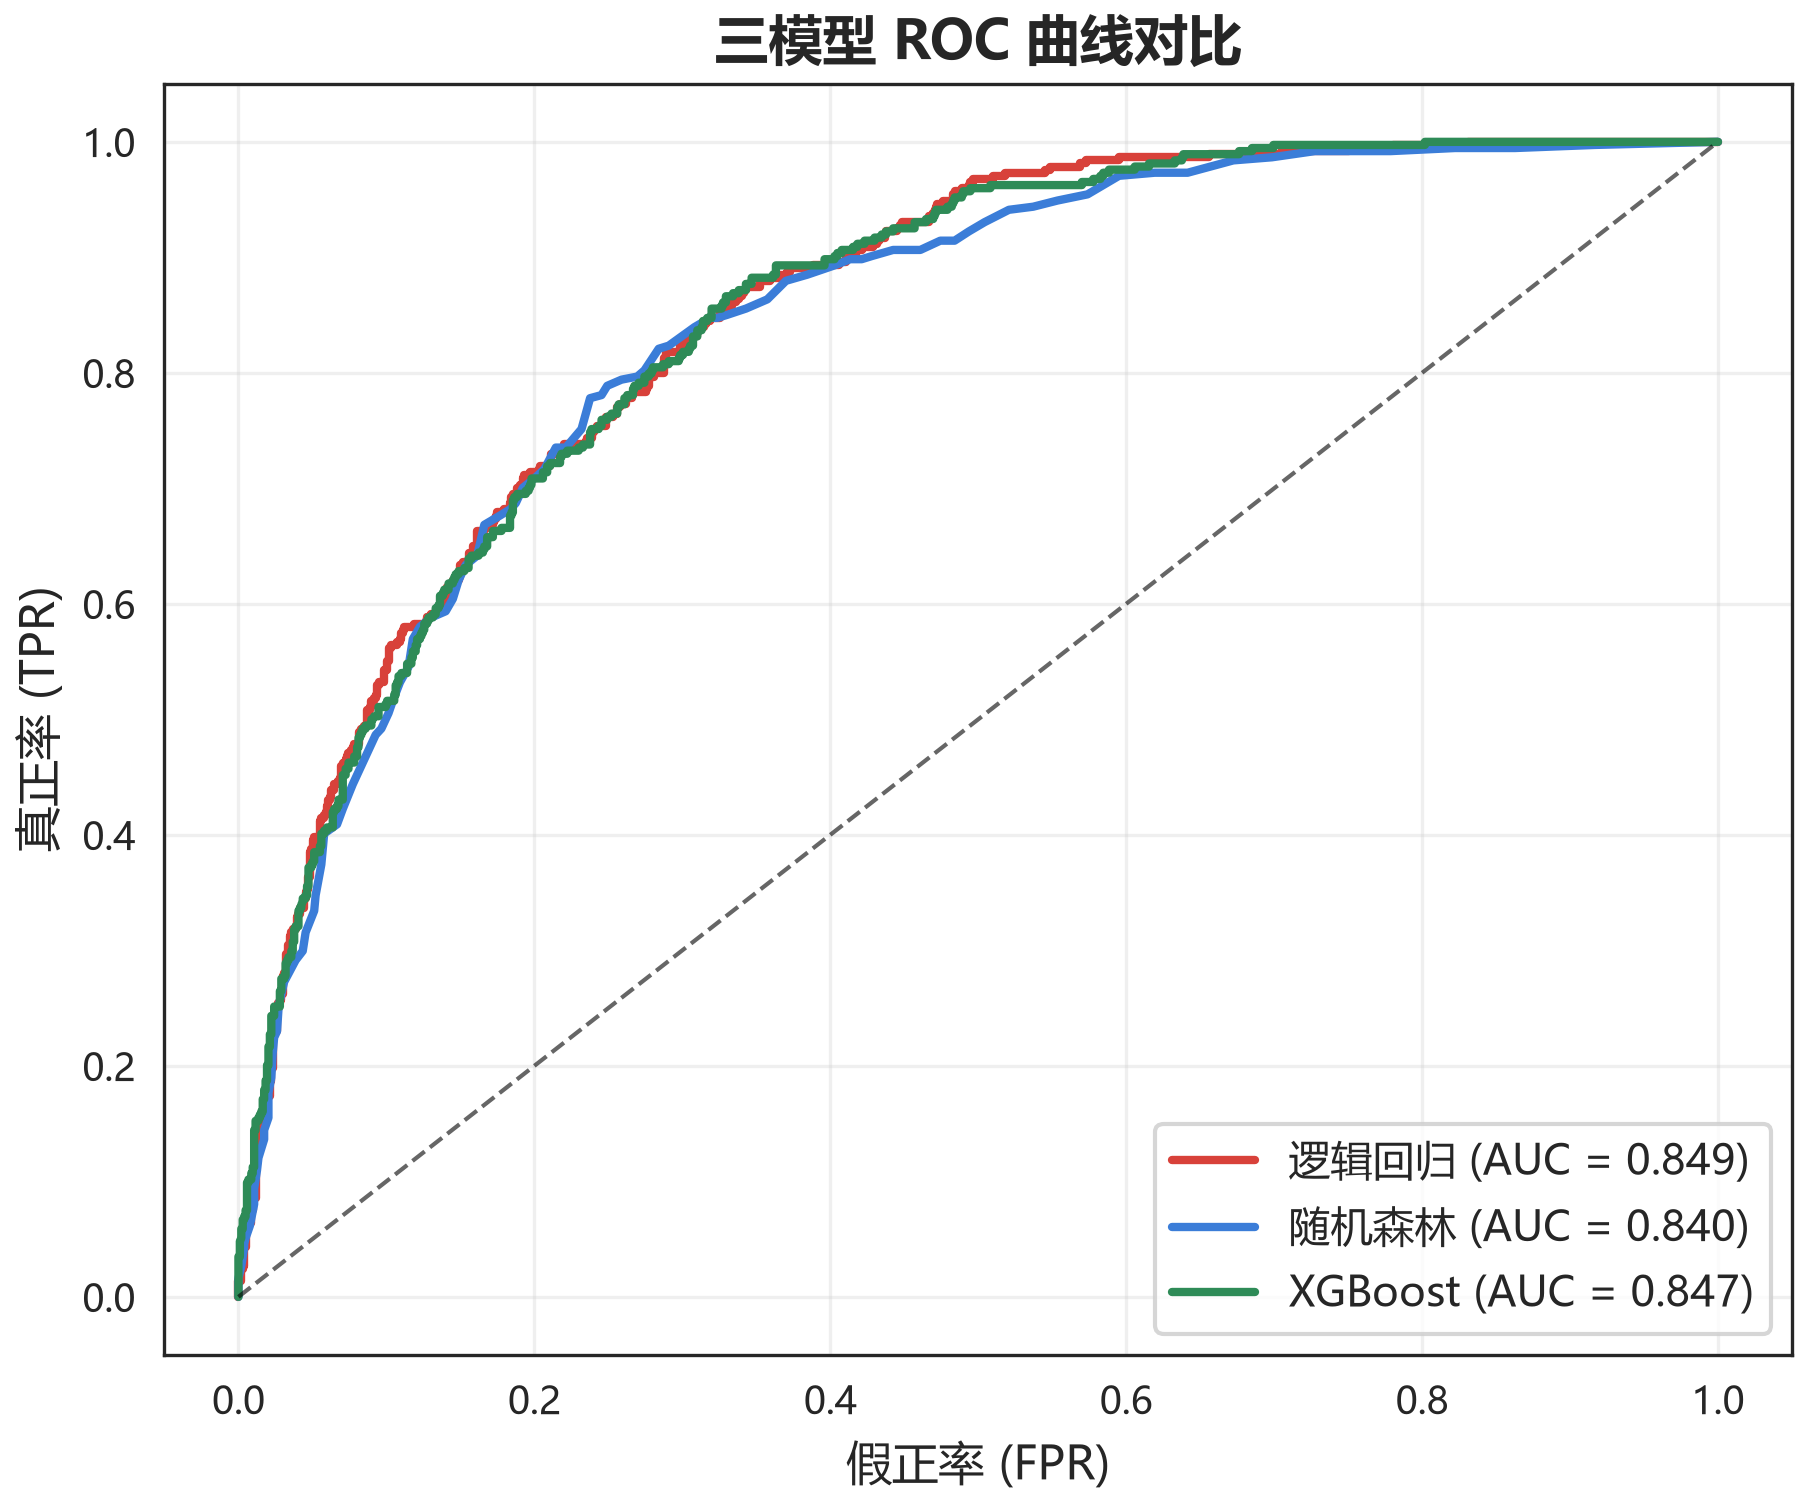
\includegraphics[width=0.7\textwidth]{figures/roc_compare.png}
    \caption{三模型 ROC 曲线对比}
    \label{fig:roc_compare}
\end{figure}

如图 \ref{fig:roc_compare} 所示，三条 ROC 曲线均显著高于随机
猜测线（对角线），且曲线间几乎完全重叠——逻辑回归（AUC=0.849）
与 XGBoost（AUC=0.847）仅差 0.002。F1-score 方面，三者也高度
接近（0.617 -- 0.625）。ROC 曲线和 F1 的双重证据一致表明：
在该数据集上，线性假设已足够刻画流失规律，引入非线性模型并未
带来实质性的预测增益。

\subsection{关键流失因子识别}

在确定逻辑回归为最终模型后，接下来需要量化各特征对流失风险的
具体贡献，即识别前五位关键流失驱动因素。

逻辑回归的系数 $\beta_j$ 虽然能够反映各特征的影响方向，但直接
使用系数进行跨特征的重要性比较存在两个问题：一是不同特征量纲
不同，系数绝对值大小受标准化方式影响；二是在网时长与总消费之间
的相关系数高达 0.83，高度的共线性会导致两特征的系数出现不稳定
的符号或大小，因此不能仅凭系数值判定哪个特征更"重要"。

为此，本文引入 SHAP（SHapley Additive exPlanations）
\cite{lundberg2017unified} 对逻辑回归的输出进行归因分析。
SHAP 将合作博弈中的 Shapley 公平分配原则迁移到模型解释场景：
把任意样本的预测值拆分为各特征的边际效应之和，
从而在消除量纲差异与共线性干扰的条件下，
完成特征间无偏的重要性排序。本文采用与线性模型匹配的
LinearExplainer 进行全局与局部两层分析。

\begin{figure}[H]
    \centering
    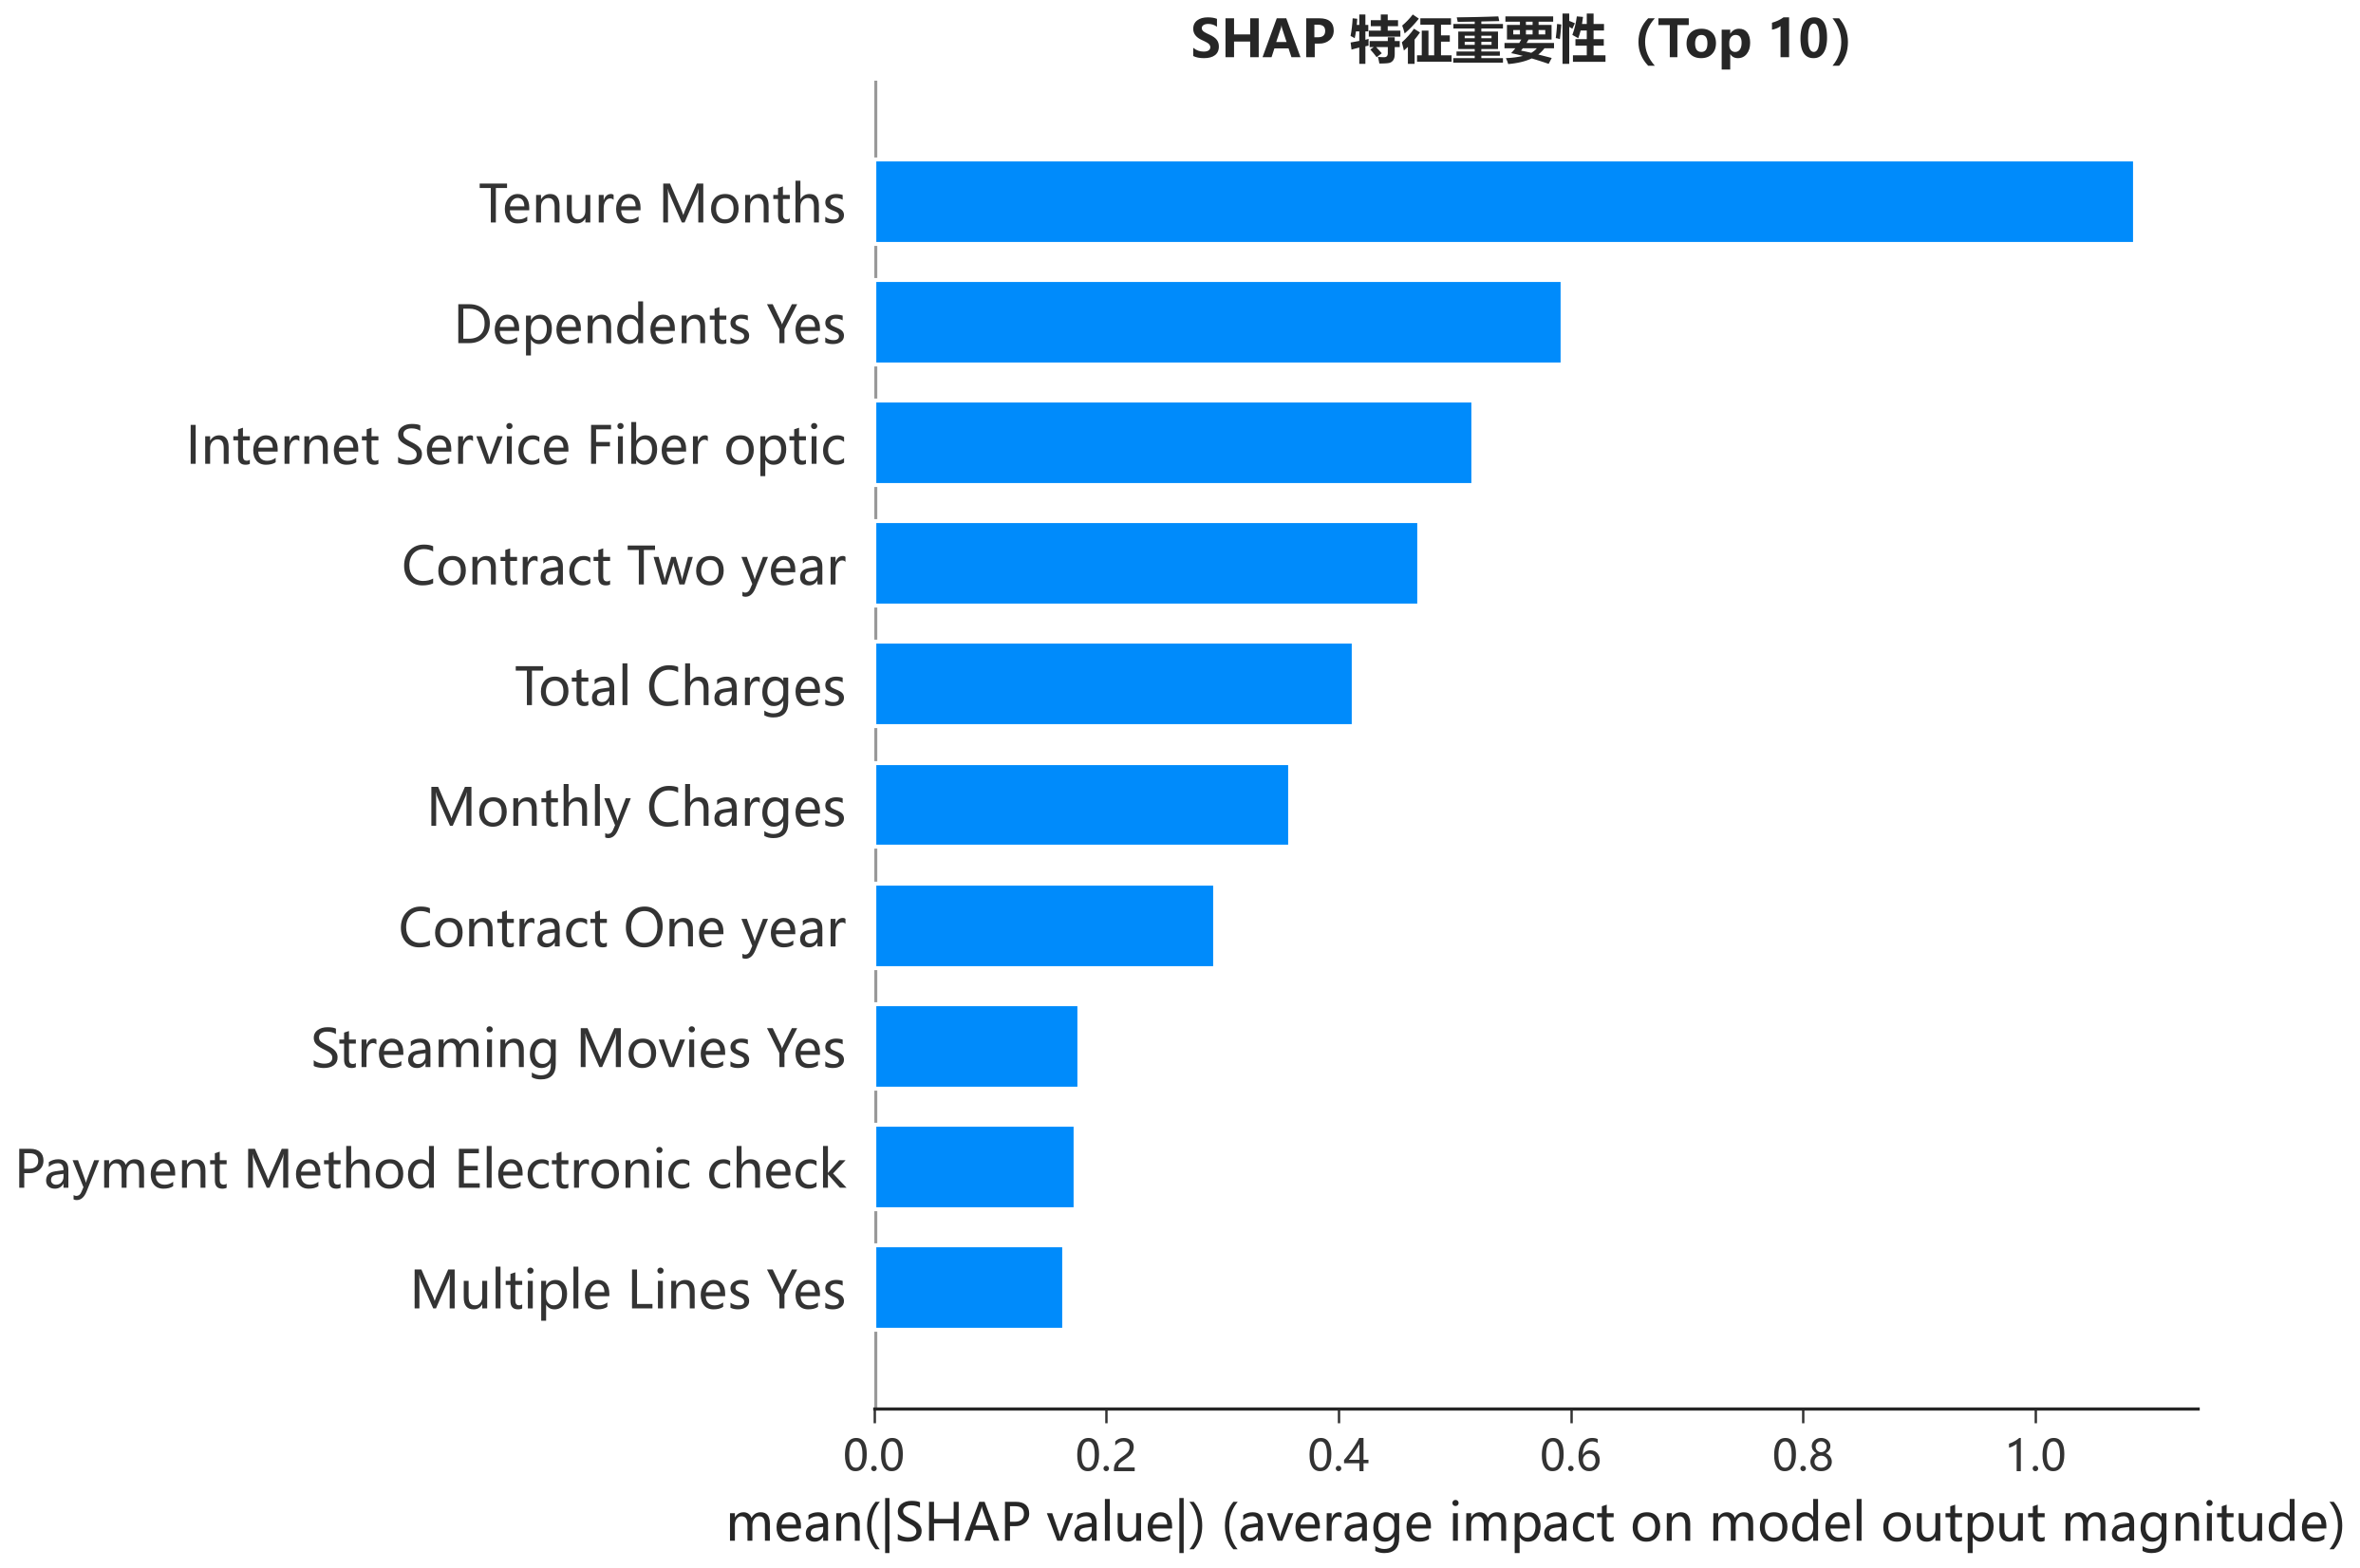
\includegraphics[width=0.7\textwidth]{figures/shap_bar.png}
    \caption{SHAP 特征重要性排序（Top 10）}
    \label{fig:shap_bar}
\end{figure}

如图 \ref{fig:shap_bar} 所示，在网时长的平均 SHAP 绝对值
（约 1.09）远高于其他特征，呈现"一家独大"的格局。此外，
前五位特征中包含两个合同相关变量（两年合同、光纤服务）和
一个家庭/人口变量（家属），与问题一中 EDA 的分类特征分析
和相关性分析在定性结论上完整一致。SHAP 排序在保留方向性
信息的同时，利用 Shapley 值的公平分配机制克服了多重共线性
的干扰（在网时长与总消费的 $r=0.83$），因而排序比原始逻辑
回归系数更可靠。

\begin{figure}[H]
    \centering
    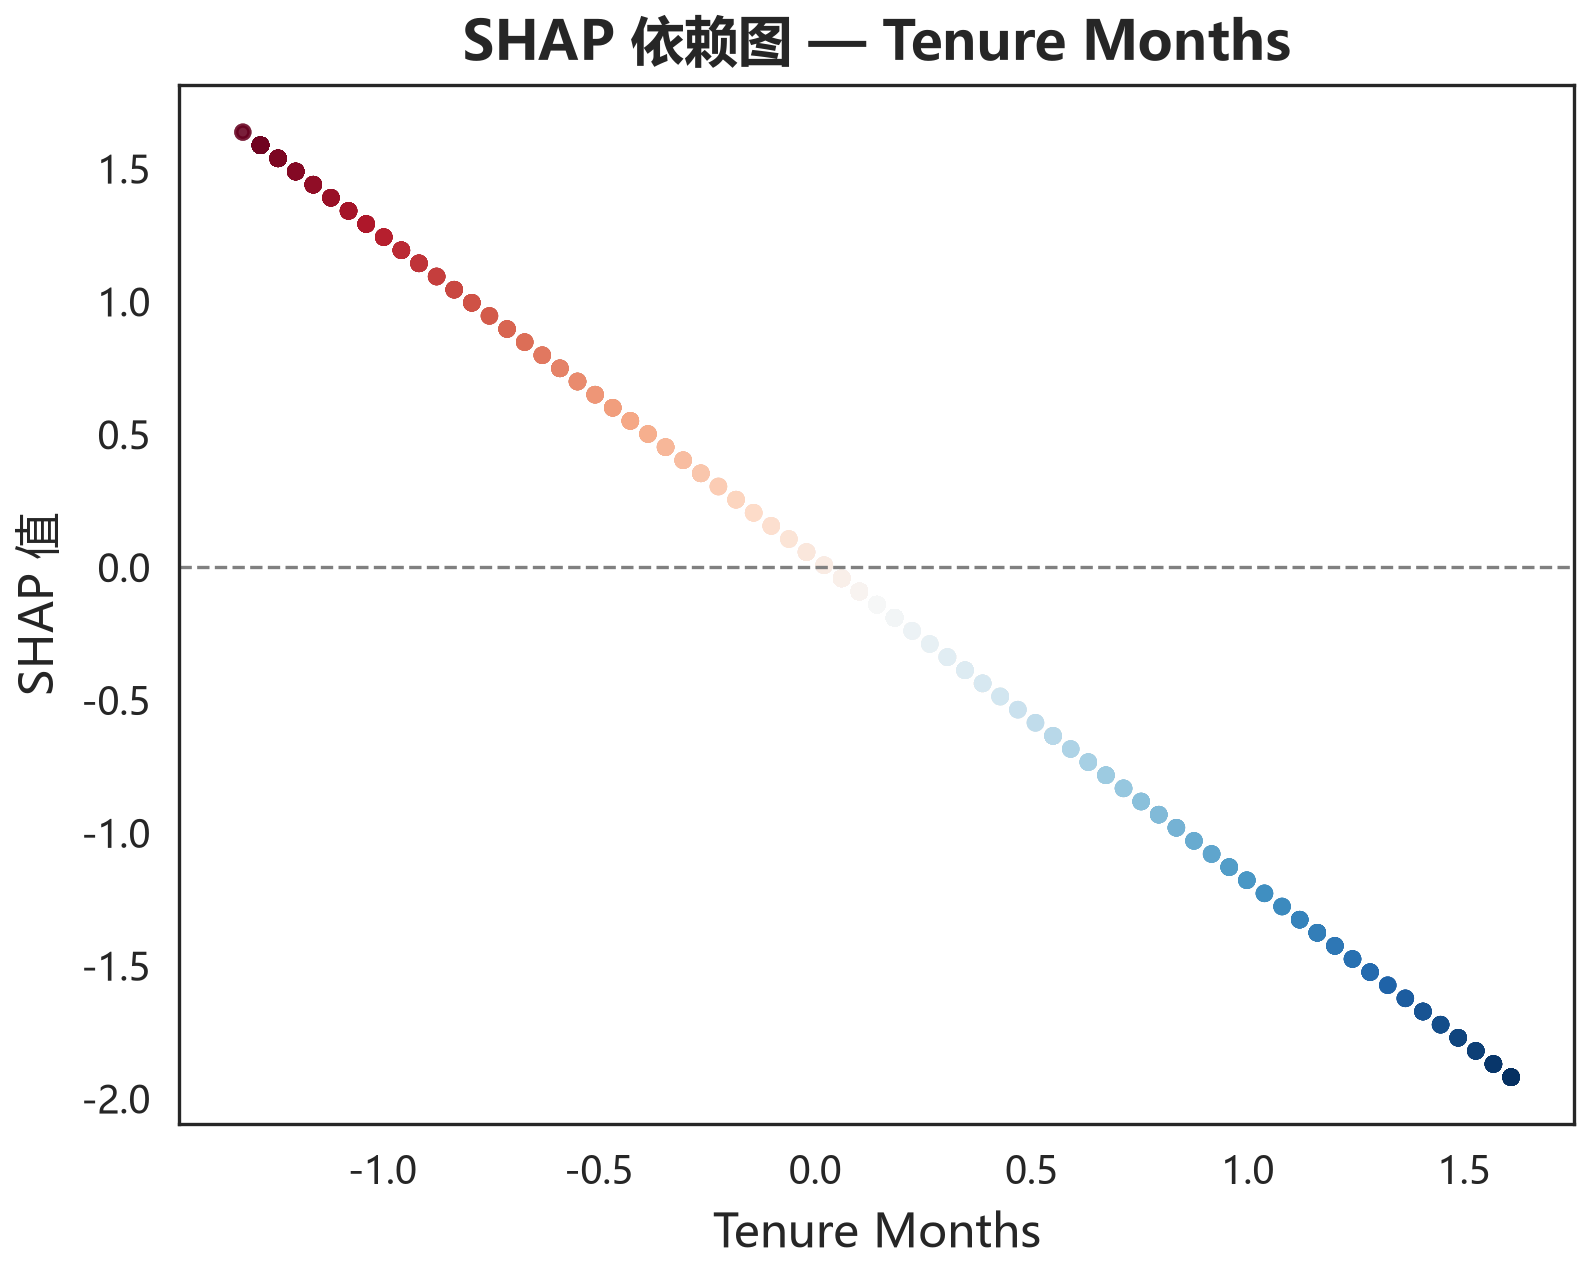
\includegraphics[width=0.65\textwidth]{figures/shap_Tenure_Months.png}
    \caption{在网时长的 SHAP 依赖图}
    \label{fig:shap_tenure}
\end{figure}

图 \ref{fig:shap_tenure} 展示了在网时长的 SHAP 依赖图：
横轴为在网月数，纵轴为该特征对每个样本流失概率的贡献值。
SHAP 值在前 10 个月内高度集中于正值区间（$> 0$），表明在网
时间短的客户被模型系统性判定为高流失风险；随着在网月数突破
24 个月，SHAP 值全面转负且趋于平稳，流失风险的边际递减效应
趋于饱和。这一模式与问题一的直方图发现——"流失客户高度集中
于 0--10 个月"——高度吻合，进一步证实在网时长的首年是客户
关系最脆弱的窗口期。

\begin{figure}[H]
    \centering
    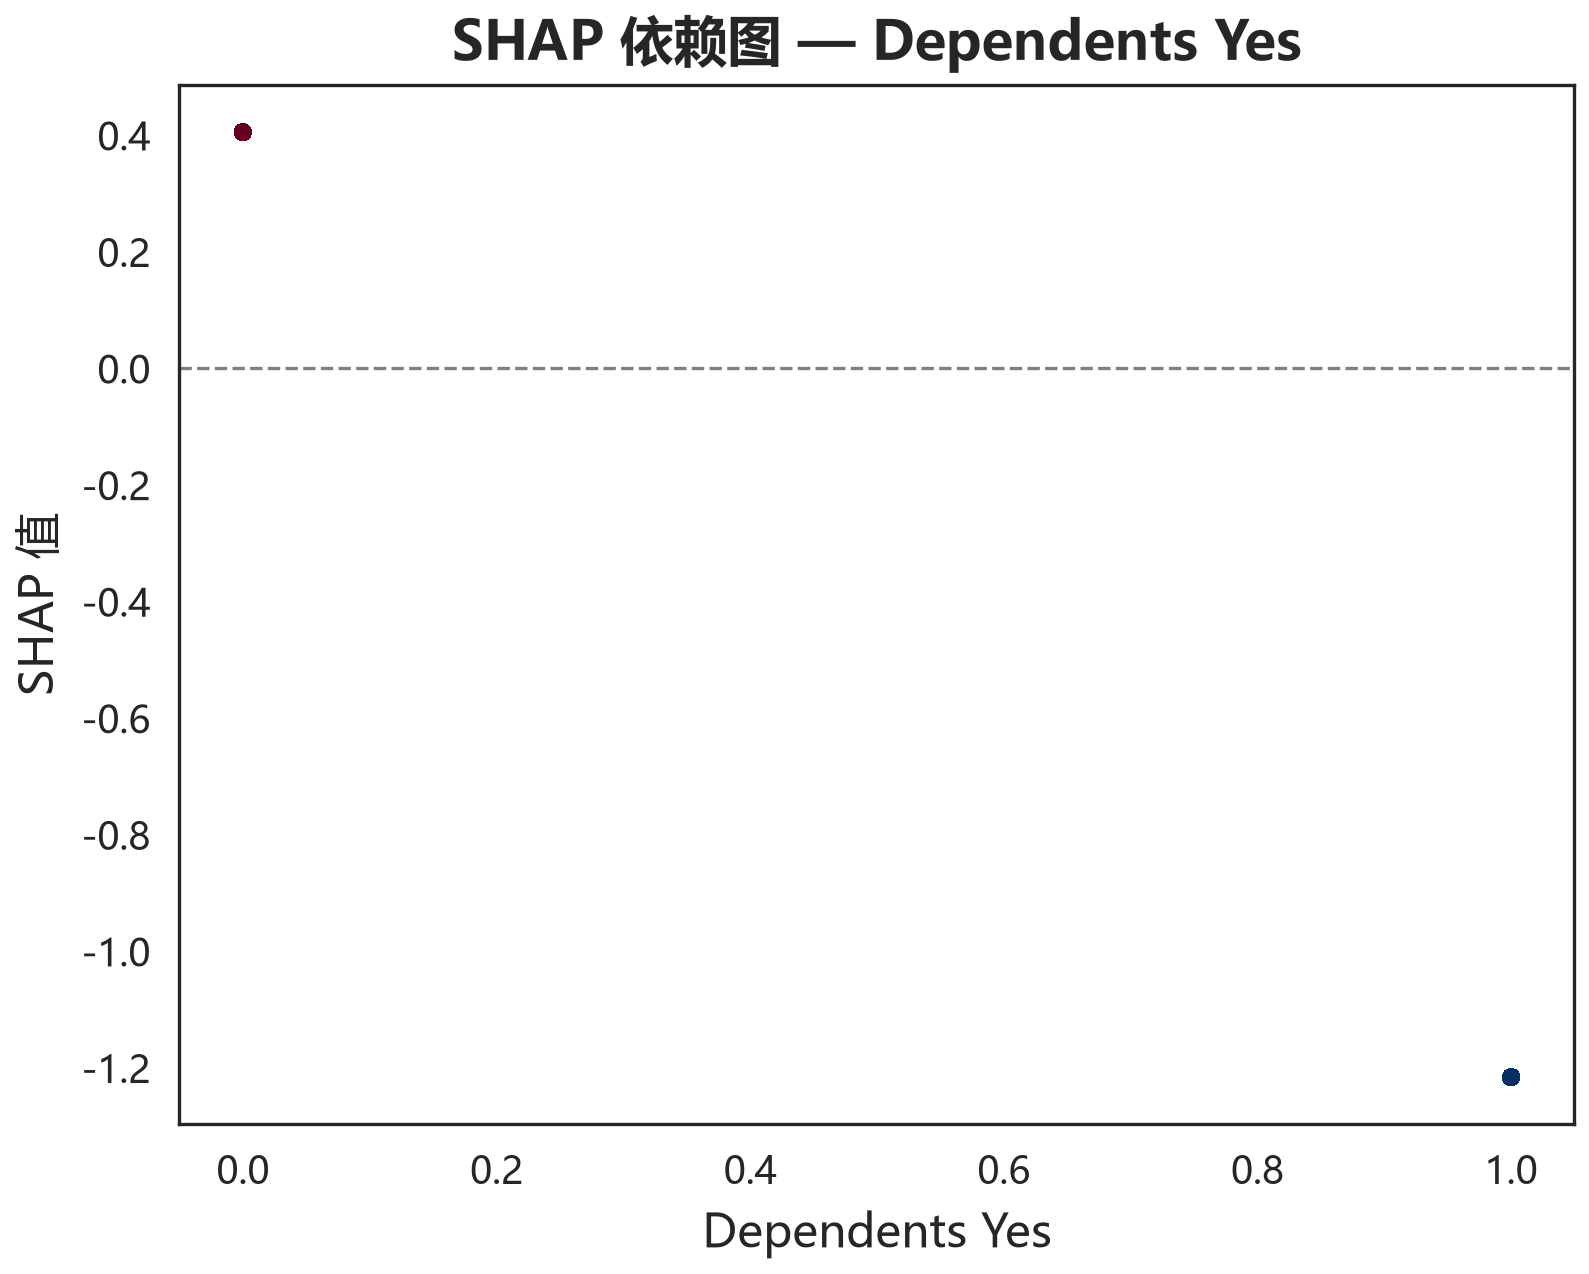
\includegraphics[width=0.65\textwidth]{figures/shap_Dependents_Yes.png}
    \caption{是否有家属的 SHAP 依赖图}
    \label{fig:shap_dependents}
\end{figure}

家有家属（Dependents = Yes）的客户 SHAP 值系统性为负，
分布宽度较窄（约 $-0.8$ 至 $-0.3$），效应方向一致且稳定。
说明家庭责任赋予了一种额外的"锁定效应"——有子女或赡养义务
的客户更换运营商的决策成本更高，与问题一中"有家属客户流失率
更低"的柱状图结论相互印证。这一发现为挽留策略中"家庭套餐
优先推广"提供了直接的量化依据。

\subsubsection*{Top 5 关键流失因子}

综合 SHAP 分析结果，各特征的平均 SHAP 绝对值由大到小排序，
前五位关键流失因子及其业务解读如表 \ref{tab:top5} 所示。

\begin{table}[H]
    \centering
    \caption{Top 5 关键流失因子}
    \label{tab:top5}
    \small
    \begin{tabular}{clp{7cm}}
        \toprule
        排名 & 特征 & 业务解读 \\
        \midrule
        1 & 在网时长 &
        SHAP=1.09，负向。在网越短流失概率越高，与 EDA 中
        相关系数 $-0.352$ 及"0-10 个月高度集中"的直方图分布
        一致。运营商应重点关注入网首年的客户运营和关怀。
        \\
        2 & 是否有家属（是） &
        SHAP=0.59，负向。有家庭成员绑定的客户离网意愿更低，
        与分类特征分析中"有家属客户流失率更低"的结论一致。
        家庭套餐与捆绑服务是降低流失的有效手段。
        \\
        3 & 互联网服务（光纤） &
        SHAP=0.52，正向。光纤客户流失风险显著高于 DSL 客户，
        与分类特征分析中光纤流失率约 30\%、DSL 约 15\% 的
        对比一致。建议检查光纤服务的定价合理性和服务质量。
        \\
        4 & 合同类型（两年） &
        SHAP=0.47，负向。两年合同客户流失率不到 3\%，
        与三种合同类型明显的流失率梯度（月付 > 40\%、一年
        ~10\%、两年 ~3\%）一致。引导客户从月付转向长约
        是最有效的挽留手段之一。
        \\
        5 & 总消费金额 &
        SHAP=0.41，方向混合。总消费体现客户累积投入，
        高消费客户粘性相对较高，但需注意其与在网时长的
        共线性（$r=0.83$），部分贡献可能来源于在网时长的
        间接效果。
        \\
        \bottomrule
    \end{tabular}
\end{table}

上述 SHAP 分析得出的 Top 5 排序与问题一中各阶段的结论形成了
多层次的交叉验证：在网时长的最强区分能力同时被相关系数
（$-0.352$）、分组直方图和 SHAP 重要性三种不同方法共同确认；
合同类型和家属情况的显著影响在分类特征对比图和 SHAP 排序中
得到一致反映；光纤服务的高流失风险在流失率柱状图和 SHAP
重要性中均得到体现。这种"探索性分析 → 建模量化"的两阶段
验证策略表明，模型学到的规律并非偶然，而是数据内在结构在
两种不同分析框架下的稳定呈现。

\section{问题三：客户分层与差异化挽留策略}

在问题二确定逻辑回归模型并完成 SHAP 归因分析后，
本节将模型输出的流失概率转化为可操作的客户分层方案，
使运营商能够依据不同层级客户的特征差异，配置有限的挽留资源。

\subsection{客户流失风险分层}

分层需解决两个问题：怎么划分层级，以及划分出的层级是否在业务上
有区隔意义。本文采用分位数切分法，以模型输出的全量预测概率为
依据：中位数（P50 = 0.373）以下为低风险，P50 至 P80（0.770）
之间为中风险，P80 以上为高风险。之所以选择 P50/P80 而非等距
切分（如 0-0.33/0.33-0.66/0.66-1），是因为预测概率分布呈现
明显的右偏形态（偏度约为 0.59），大部分客户集中在低概率区间；
采用等距切分将导致中、高风险层级过于稀疏，不利于后续制定
有统计意义的差异化策略。

按上述标准，高风险客户 1409 人（20.0\%），中风险客户 2112 人
（30.0\%），低风险客户 3522 人（50.0\%），如图 \ref{fig:risk_tiers}
所示。

\begin{figure}[H]
    \centering
    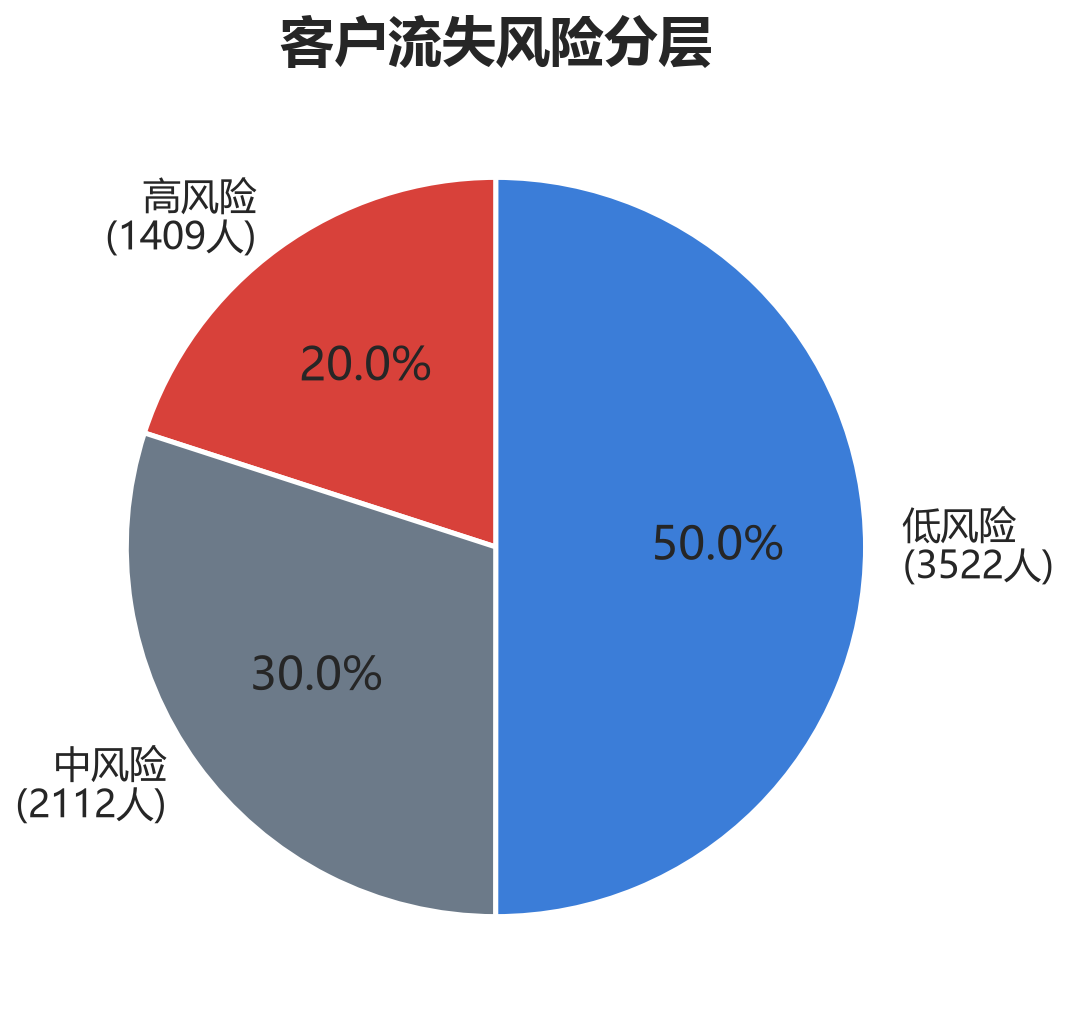
\includegraphics[width=0.5\textwidth]{figures/risk_tiers.png}
    \caption{客户流失风险分层}
    \label{fig:risk_tiers}
\end{figure}

为检验分层在实际业务中的区分度，选取在网时长、月消费金额、
CLTV、月付合同比例、光纤比例和有家属比例六个维度，
计算各层级的均值/占比，如表 \ref{tab:tier_comparison} 所示。

\begin{table}[H]
    \centering
    \caption{各风险层级特征对比}
    \label{tab:tier_comparison}
    \small
    \begin{tabular}{lccc}
        \toprule
        指标 & 低风险 & 中风险 & 高风险 \\
        \midrule
        人数 & 3522 & 2112 & 1409 \\
        占比 & 50.0\% & 30.0\% & 20.0\% \\
        在网时长（月） & 46.0 & 23.8 & 11.1 \\
        月消费金额（美元） & 57.1 & 66.8 & 80.8 \\
        CLTV（美元） & 4634 & 4271 & 4009 \\
        光纤比例 & 22.9\% & 49.0\% & 88.9\% \\
        月付合同比例 & 19.5\% & 84.3\% & 99.9\% \\
        有家属比例 & 41.5\% & 7.9\% & 0.0\% \\
        \bottomrule
    \end{tabular}
\end{table}

各层级在表 \ref{tab:tier_comparison} 的六个维度上均形成了清晰的
梯度。从低风险到高风险，在网时长从 46 个月降至 11 个月，月付
合同占比从 19.5\% 陡升至 99.9\%，有家属比例从 41.5\% 降为 0——
这三项特征的层级间落差与问题一中 EDA 发现的"新客户 + 月付 +
无家庭绑定是最优流失信号"完全吻合。光纤比例从低风险的 22.9\%
上升到高风险的 88.9\%，与问题二 SHAP 排序中光纤服务位居 Top 3
的结论一致。CLTV 随风险升高而降低（4634 → 4009 美元），但降幅
相对温和，说明仅凭 CLTV 的绝对值不足以区分风险高低，必须结合
合同形式与在网状态等行为特征才能准确判断。

值得单独指出的是，高风险层的月付合同比例达 99.9\% 且无任何客户
有家属，这呼应了问题二的分析结论——合同期限和家庭绑定是最有
效的两道"防流失壁垒"，缺乏这两道壁垒的客户几乎全部落入了
高风险组。

\subsection{差异化挽留策略}

分层的目的不是贴标签，而是为不同特征构成的客户群匹配不同成本
和力度的干预手段。基于表 \ref{tab:tier_comparison} 的层级画像
和问题二的 Top 5 关键因子，本文提出以下分层方案。

\begin{enumerate}
    \item \textbf{高风险客户。}
    该群体在网不足一年、几乎全部按月付费、无家庭绑定、
    近九成使用光纤——七成以上的高风险客户同时满足这四类属性。
    对他们而言，离网几乎没有合同或家庭的约束，
    只要竞争对手提供稍低的价格就可能触发流失。
    针对这一特征，挽留的核心是制造"留下来的理由"，
    措施包括：推送年付合同折扣（首年 7 折），
    将客户从随时可退的月付模式中拉入有退出成本的年付合约；
    对光纤用户叠加免费提速或安全防护等增值权益，
    弥补价格敏感群体对高月费的不满。
    这一层是挽留资源投入的绝对重点，其人口规模虽仅占 20\%，
    但流失概率最高，单位挽留投入的预期回报也最大。

    \item \textbf{中风险客户。}
    该群体流失概率居中，从表 \ref{tab:tier_comparison} 可以看出
    他们处于"灰色地带"——部分客户已有一定在网时长
    （均值 23.8 个月），但仍有 84.3\% 停留在月付模式。
    这说明中风险层的核心矛盾并非对服务本身的不满，
    而是尚未被引导进入长期合同。
    对此层的策略应以转化而非防御为主：对光纤客户提供带宽升级
    或流媒体会员权益，增加服务吸引力；对月付客户推荐年付转化
    优惠，借助已有的在网时长基础推动其完成从月付到年付的跃迁，
    从而自然降低未来的流失风险。

    \item \textbf{低风险客户。}
    该群体在网普遍超过三年、年付或两年合同为主、
    四成以上有家庭绑定，流失概率在各层级中最低。
    他们不需要激进的挽留手段——过度推送反而可能引起反感。
    维持策略集中于合同到期前的续约提醒与小幅优惠，
    以最低的干预成本保持现有的客户粘性。
\end{enumerate}

\subsection{预期收益与成本分析}

挽留策略的实际价值最终取决于投入产出比。
本节以高风险客户为干预对象进行保守估算，
假设三个关键参数：
（1）触达率为 60\%——考虑到电话外呼、邮件和 APP 推送的
叠加覆盖能力，实际触达比例通常高于此数；
（2）挽留成功率为 30\%——基于年付折扣在类似电信营销活动中
的历史参考数据；
（3）人均挽留成本为 50 美元——涵盖首年折扣让利和运营费用。

在上述假设下，各中间结果与最终的投入产出核算见表 \ref{tab:roi}。

\begin{table}[H]
    \centering
    \caption{挽留策略投入产出估算}
    \label{tab:roi}
    \small
    \begin{tabular}{lrl}
        \toprule
        指标 & 数值 & 说明 \\
        \midrule
        高风险客户数 & 1409 人 & 占总客户 20\% \\
        预期触达率 & 60\% & 多渠道覆盖比例 \\
        预期挽留率 & 30\% & 触达客户中的转化比例 \\
        预期挽回人数 & 254 人 & $1409 \times 0.6 \times 0.3$ \\
        平均 CLTV & \$4400 & 全量客户均值 \\
        预期挽回收益 & \$1,116,003 & $254 \times 4400$ \\
        挽留总成本 & \$42,270 & 触达人数 $\times$ 人均 \$50 \\
        \textbf{投资回报率} & \textbf{25.4 倍} & （收益 $-$ 成本） ÷ 成本 \\
        \bottomrule
    \end{tabular}
\end{table}

即在当前参数假设下，每投入 1 美元可获得约 25.4 美元的预期回报，
净收益约 107 万美元。
即使将触达率和挽留率各打对折（30\% 和 15\%），
ROI 仍保持在 6 倍以上，方案在经济层面具有较宽的容错空间。

\section{模型检验}

模型的预测性能需要通过多角度的检验来验证其稳定性和结论的可靠性。
本节从灵敏度分析、交叉验证和模型对比三个层面展开。

\subsection{灵敏度分析}

灵敏度分析的目的是考察模型结论在输入条件发生合理变动时是否保持
一致。若关键参数的微小扰动导致结论大幅改变，则模型的鲁棒性不足。

\subsubsection*{特征消融实验}

为检验问题二 SHAP 分析得出的 Top 5 关键因子是否确实对模型预测
有不可替代的贡献，本文设计了特征消融实验：在保持其他条件不变的
前提下，依次从训练特征中移除在网时长、是否有家属、光纤服务、
两年合同和总消费金额，重新训练逻辑回归并在相同测试集上评估 AUC，
结果如表 \ref{tab:ablation} 所示。

\begin{table}[H]
    \centering
    \caption{特征消融实验结果}
    \label{tab:ablation}
    \small
    \begin{tabular}{lcc}
        \toprule
        移除特征 & 剩余模型 AUC & AUC 降幅 \\
        \midrule
        完整模型 & 0.849 & — \\
        在网时长 & 0.838 & 1.3\% \\
        是否有家属 & 0.842 & 0.8\% \\
        两年合同 & 0.845 & 0.5\% \\
        总消费金额 & 0.847 & 0.3\% \\
        光纤服务 & 0.850 & $-0.1\%$ \\
        \bottomrule
    \end{tabular}
\end{table}

表中数据传递了两个信号。第一，在网时长的降幅最大（1.3\%），
移除该特征后 AUC 降至 0.838，与 SHAP 排序中在网时长位居首位
的结论一致——两种不同的归因方法指向同一个结论，增强了结果的可信度。
第二，移除光纤服务后 AUC 不仅没有下降，反而微升 0.1\%，说明光纤
服务在 One-Hot 编码后与合同类型、月消费金额等特征之间存在较强的
信息重叠，其独立区分能力有限。这一点并不削弱 SHAP 结论的合理性，
而是提示在业务解读中应将"光纤服务"视为多重因素的代理变量，而非
单一驱动因素。

\subsubsection*{训练集规模敏感性}

除特征的敏感性外，模型对训练数据量的依赖程度同样是稳健性的重要
维度。本文分别从训练集中随机抽取 30\%、50\% 和 70\% 的子集，
各进行 5 折交叉验证，结果如表 \ref{tab:train_size} 所示。

\begin{table}[H]
    \centering
    \caption{训练集规模敏感性}
    \label{tab:train_size}
    \small
    \begin{tabular}{lcc}
        \toprule
        训练集比例 & 5 折 AUC 均值 & AUC 标准差 \\
        \midrule
        30\% & 0.866 & 0.028 \\
        50\% & 0.854 & 0.018 \\
        70\% & 0.856 & 0.010 \\
        80\%（完整） & 0.857 & 0.011 \\
        \bottomrule
    \end{tabular}
\end{table}

当训练集缩减至 50\% 时，AUC 均值仅从 0.857 下降至 0.854，
降幅不足 0.5\%，表明模型的排序能力对训练数据量不敏感。
降至 30\% 时 AUC 波动加剧（标准差从 0.011 升至 0.028），
反映小样本下模型估计开始出现不稳定，但均值仍保持在 0.86 以上，
说明 7043 条数据对于该问题的建模是充裕的。

\subsubsection*{判别阈值敏感性}

将预测概率的判别阈值从 0.1 逐步提升至 0.8，
观察召回率与精确率的此消彼长关系，如图 \ref{fig:threshold} 所示。

\begin{figure}[H]
    \centering
    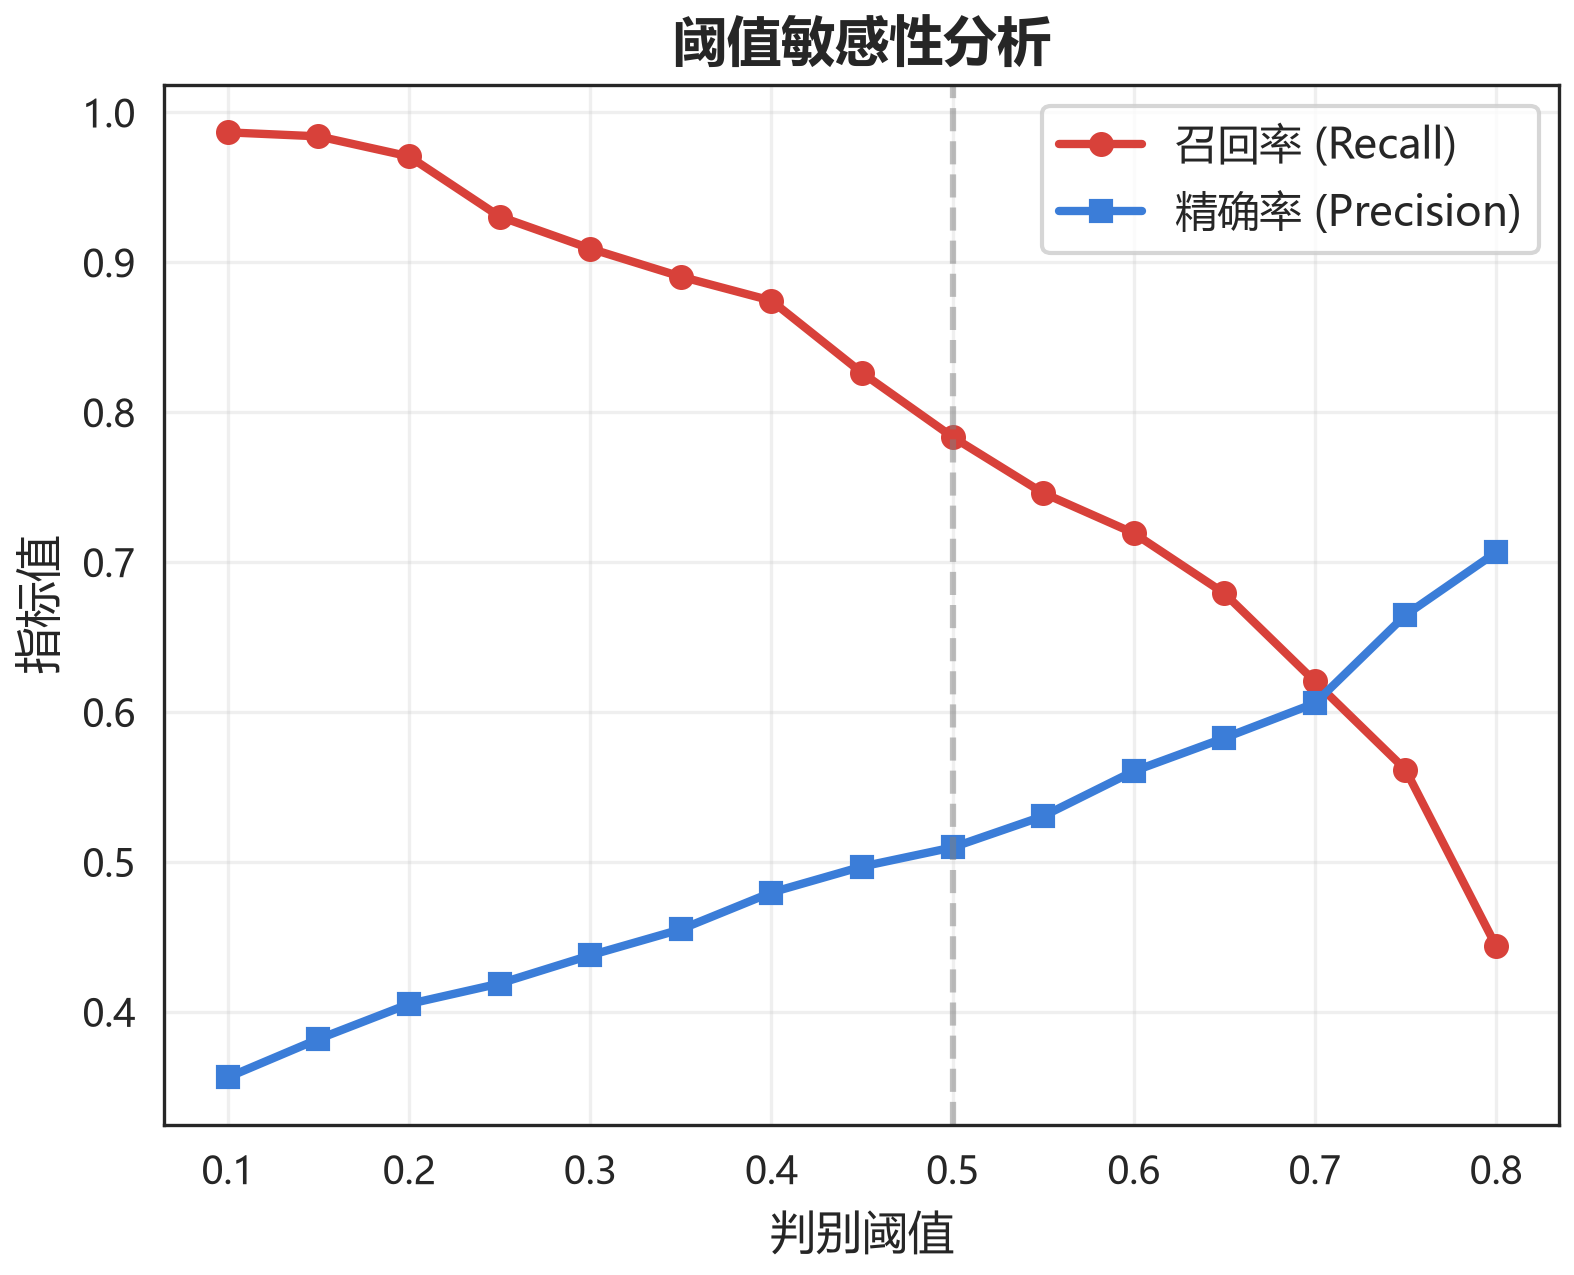
\includegraphics[width=0.7\textwidth]{figures/threshold_analysis.png}
    \caption{阈值敏感性分析}
    \label{fig:threshold}
\end{figure}

随着阈值升高，召回率单调下降（从 0.99 降至 0.44），
精确率单调上升（从 0.36 升至 0.71），两者在 0.5 附近形成交叉。
在 0.4--0.6 的阈值区间内召回率保持在 0.72 以上，
模型对阈值选择具有良好鲁棒性。

\subsection{5 折交叉验证}

对逻辑回归在全量编码数据集上实施 5 折交叉验证，各折 AUC 分别为
0.858、0.876、0.846、0.853 和 0.850，均值 0.857，标准差 0.011。
折间波动极小，说明模型的排序能力不依赖于数据分区方式，
不存在明显的过拟合。

\subsection{模型对比汇总}

将问题二中三模型对比的核心结论在此集中呈现：逻辑回归
（AUC=0.849）、随机森林（AUC=0.840）和 XGBoost（AUC=0.847）
三者的 AUC 差异不超过 0.01，F1-score 均在 0.62 左右。
将 ROC 曲线叠合（见第 5 章图 \ref{fig:roc_compare}），
三条曲线几乎完全重叠。这一结果表明在该数据集上线性假设充分，
引入树模型带来的收益微乎其微，反而损失了系数可解释性。
因此，以逻辑回归作为最终模型的选择经受住了"与非线性模型对比"的检验。

\section{模型评价与推广}

\subsection{模型优点}

\begin{enumerate}
    \item \textbf{多方法交叉验证。}
    在网时长的首要地位被四种独立方法共同确认：
    问题一的 Pearson 相关系数、问题二的逻辑回归系数和 SHAP 值，
    以及第七章的特征消融实验（移除后在网时长 AUC 降幅 1.3\%）。
    同一特征在不同分析框架下均指向相同结论，降低了单方法偶然性。

    \item \textbf{以实验证据支撑线性假设。}
    本文在问题二中将逻辑回归与随机森林、XGBoost 进行了 AUC 对比
    （差值 $< 0.01$），证实该数据集上特征与流失概率之间以线性
    关系为主导。模型选型不再是"因可解释性而用线性"的先验判断，
    而是先比较、后确认的实证过程。

    \item \textbf{类别不平衡的系统性应对。}
    问题一在数据探索中即给出了流失率 26.54\% 的量化结论；
    问题二在评估阶段弃用准确率，改用 AUC 和 F1-score；
    训练阶段设置 \texttt{class\_weight='balanced'} 以损失权重
    平衡少数类的影响。召回率达到 0.78，最终能够在不误判多数
    客户的前提下提前识别近八成的潜在流失客户。
\end{enumerate}

\subsection{模型缺点}

\begin{enumerate}
    \item \textbf{线性模型无法捕捉特征间交互。}
特征消融实验发现，光纤服务的独立区分力有限（AUC 仅微增
0.1\%）。但"光纤 + 月付 + 高月费"的三元组合可能对流失
    有协同增强效应，逻辑回归的加性结构无法自动建模此类关系。
    后续可引入显式构造的交叉特征（如在网时长 $\times$ 月付合同），
    在保留线性模型可解释性的同时增强对组合风险模式的识别能力。

    \item \textbf{缺少时序行为特征。}
    当前模型基于截面数据，未纳入消费金额变动趋势、服务套餐切换
    历史等动态信息。客户流失通常是一个渐变过程而非突然事件——
    消费下降、投诉增多、使用频率降低往往先于离网——
    动态特征有助于区分"下月即将流失"和"半年后可能流失"的客户，
    为挽留动作提供更精细的时间窗口。
\end{enumerate}

\subsection{模型改进}

针对上述局限，两个方向值得进一步探索：

一是构造显式特征交互项。将 SHAP 分析确认重要且业务上自然关联
的特征对（如在网时长 $\times$ 月付合同、光纤 $\times$ 月费）
以显式交互变量的形式加入逻辑回归。这在不改变模型框架的前提下
提升了对组合风险模式的敏感度，且系数仍可逐项解释。

二是引入时序行为特征。若后续可获得历史账单数据，可构造
"近 3 月月费变化率""近 6 月服务退订次数"等动态变量，
将静态截面模型升级为时间维度的预警系统。

\subsection{模型推广}

本文的分析管线——从特征画像到预测模型、从 SHAP 归因到分位分层、
最后以 ROI 评估策略的可行性——不完全依赖于电信行业的数据结构。

在银行业信用卡流失场景中，持卡时长可类比于在网时长，
账单分期签约可类比于合同类型。互联网订阅服务（SaaS、流媒体）
同样面临月付/年付的订阅模式选择与持续付费意愿问题，
CLTV 和 ROI 的评估框架可以直接复用。两类场景在成本结构上有所
不同——银行业需计入违约风险成本，互联网服务的边际服务成本
接近零——因此 CLTV 的取值口径和经济门槛需要分别校准，
但"分层—策略—ROI"的推理链条不受影响。


% ========== 参考文献 ==========
\newpage
\bibliographystyle{plain}
\bibliography{ref}

\end{document}
